
%\newtheorem{definition}[subsection]{Definition}
%\newtheorem{example}[subsection]{Example}
%\newtheorem{cor}[subsection]{Corollary}
\newtheorem{pro}[subsection]{Proposition}
\newtheorem{theo}[subsection]{Theorem}
\newtheorem{lem}[subsection]{Lemma}
%\newtheorem{rem}[subsection]{Remark}

\definecolor{main}{HTML}{5989cf}    % setting main color to be used
\definecolor{sub}{HTML}{cde4ff}     % setting sub color to be used

\tcbset{
    sharp corners,
    colback = white,
    before skip = 0.2cm,    % add extra space before the box
    after skip = 0.5cm      % add extra space after the box
}                           % setting global options for tcolorbox

% You can copy any following box you like to your code.
\newtcolorbox{boxA}{
    fontupper = \bf,
    boxrule = 1.5pt,
    colframe = black % frame color
}

\newtcolorbox{boxB}{
    fontupper = \bf\color{main}, % font color
    boxrule = 1.5pt,
    colframe = main,
    rounded corners,
    arc = 5pt   % corners roundness
}
\newtcolorbox{boxC}{
    colback = sub, % background color
    boxrule = 0pt  % no borders
}

\newtcolorbox{boxD}{
    colback = sub, 
    colframe = main, 
    boxrule = 0pt, 
    toprule = 3pt, % top rule weight
    bottomrule = 3pt % bottom rule weight
}

\hypersetup{
    colorlinks=true,
    linkcolor=blue,
    filecolor=magenta,      
    urlcolor=cyan,
    pdftitle={Overleaf Example},
    pdfpagemode=FullScreen,
    }

\urlstyle{same}


\coursetitle{\mtthreeiii}{MT303}
\developers{Wyclife Rao}
\reviewers{Dr Irene Sitawa}
\modulenumber{3}
\modulename{Interpolation and Polynomial Approximation}

% courses
\thispagestyle{empty}
\begin{tikzpicture}[overlay,remember picture,font=\sffamily\bfseries]
 \draw[ultra thick,c4,name path=big arc] ([xshift=-2mm]current page.north) arc(150:285:11) coordinate[pos=0.225] (x0);
 \begin{scope}
  \clip ([xshift=-2mm]current page.north) arc(150:285:11) --(current page.north east);
  \fill[c4!50,opacity=0.25] ([xshift=4.55cm]x0) circle (4.55);
  \fill[c4!50,opacity=0.25] ([xshift=3.4cm]x0) circle (3.4);
  \fill[c4!50,opacity=0.25] ([xshift=2.25cm]x0) circle (2.25);
  \draw[ultra thick,c4!50] (x0) arc(-90:30:6.5);
  \draw[ultra thick,c4] (x0) arc(90:-30:8.75);
  \draw[ultra thick,c4!50,name path=arc1] (x0) arc(90:-90:4.675);
  \draw[ultra thick,c4!50] (x0) arc(90:-90:2.875);
  \path[name intersections={of=big arc and arc1,by=x1}];
  \draw[ultra thick,c4,name path=arc2] (x1) arc(135:-20:4.75);
  \draw[ultra thick,c4!50] (x1) arc(135:-20:8.75);
  \path[name intersections={of=big arc and arc2,by={aux,x2}}];
  \draw[ultra thick,c4!50] (x2) arc(180:50:2.25);
 \end{scope} 
 \path[decoration={text along path,text color=c4,
                 raise = -2.8ex,
                 text  along path,
                 text = {},%|\sffamily\bfseries|02/18/2019
                 text align = center,
             },
             decorate
         ] ([xshift=-2mm]current page.north) arc(150:245:11);
 %
 \newcommand\add{4cm}
 \begin{scope}%[shift={(5,0)}]
  \path[clip,postaction={fill=c3}]
  ([xshift=2cm+\add,yshift=-8cm]current page.center) rectangle ++ (4.6,7.7);
  \draw[c5,ultra thick,fill=c2] ([xshift=0.5cm+\add,yshift=-8cm]current page.center)
   ([xshift=0.5cm+\add,yshift=-8cm]current page.center)  arc(180:60:2)
    |- ++ (-3,6) --cycle;
  \draw[ultra thick,c5] ([xshift=-1.5cm+\add,yshift=-8cm]current page.center) 
  arc(180:0:2);
  \draw[ultra thick,c5] ([xshift=0.5cm+\add,yshift=-8cm]current page.center) 
  arc(180:0:2);
  \draw[ultra thick,c5] ([xshift=2.5cm+\add,yshift=-8cm]current page.center) 
  arc(180:0:2);
  \draw[ultra thick,c5] ([xshift=4.5cm+\add,yshift=-8cm]current page.center) 
  arc(180:0:2);
  \fill[white] ([xshift=2.5cm+\add,yshift=-8cm]current page.center) +(60:2) circle(1.5mm)
  node[above
  right=0mm,text=c5!80!black]{$\rho:=\dfrac{1+\sqrt{-3}}{2}$};
 \end{scope}
 %
 \fill[c1] ([xshift=2cm+\add,yshift=-8cm]current page.center) rectangle ++ (-30.7,7.7);
 \node[text=white,anchor=west,scale=2.3,inner sep=0pt] at
 ([xshift=-10cm,yshift=-1.8cm]current page.center) {\color{ulabgold} LEARNING};
 \node[text=white,anchor=west,scale=5,inner sep=0pt] at
 ([xshift=-10cm,yshift=-3.25cm]current page.center) {MODULE \dpmdnumber};
 \node[text=white,anchor=west,scale=2.5,inner sep=0pt,text width=.4\textwidth] at
 ([xshift=-10cm,yshift=-6cm]current page.center) {\dpmdname};
 \node[text=white,anchor=east,scale=2,inner sep=0pt] at
 ([xshift=5.7cm,yshift=-7.5cm]current page.center) {\color{ulabgold}The Open University of Kenya};
 %
% \draw[gray,line width=5mm] 
% ([xshift=2mm,yshift=-1mm]current page.south west) rectangle ([xshift=-2mm,yshift=1mm]current
% page.north east);
\end{tikzpicture}

%\newpage
\pagenumbering{roman}
\thispagestyle{empty}%firstpage


\begin{center}
\vspace*{2cm}
{\Huge\bf BACHELOR OF TECHNOLOGY EDUCATION}\\[3cm]  


%{\fontsize{80}{40}\selectfont \dpcoursecode}\\[2cm]
%
%{\fontsize{30}{40} \selectfont \dpcoursename}\\[2cm]

%\rule{\textwidth}{1pt}
%\vspace{2cm}

%{\fontsize{40}{40}\selectfont \bf Module~\dpmdnumber}\\[2cm]
%
%{\fontsize{30}{40}\selectfont \bf \dpmdname}\\

\vfill
\begin{flushright}
\begin{minipage}{.6\textwidth}
\begin{tcolorbox}%[text ]
\begin{tabular}{ll}%\hline
\subtitle{Developed by:}&\displaydevelopers\\
&\\
\subtitle{Reviewed by:}&\makecell[l]{\displayreviewers}\\
\end{tabular}
\end{tcolorbox}
\end{minipage}\hspace*{-3.5cm}
\end{flushright}
\vspace*{-2.5cm}
\end{center}

\newpage
\thispagestyle{empty}
\null
\vfill
{\renewcommand\arraystretch{1.5}
\begin{tabular}{|l|l|}\hline
\subtitle{Programme Title} & Bachelor of Technology Education \\\hline
\subtitle{Course Title} & \fullcoursename\\\hline
\subtitle{Learning Module number} & Module \dpmdnumber\\\hline
\subtitle{Learning module title} & \dpmdname \\\hline
\subtitle{Module Developer} & \displaydevelopers\\\hline
\subtitle{Reviewed by} & \displayreviewers\\\hline
%\subtitle{Vision} & \vision\\\hline
%\subtitle{Audience description} & \\\hline
\end{tabular}}
\clearpage

%\section{COURSE LEARNING GUIDE}


\subsection*{Preparing for Online and Distance Learning}

This course offers you the opportunity to enter an online space where you can engage with fellow students at the university. The online forums, exercises, tasks and materials have been designed by the course facilitators in such a way that you can draw directly from their knowledge and share in their scholarly interest in online learning and assessment

We hope you will use your access to this virtual classroom to raise all your questions on the course module, to build a network great learners and to share your own thoughts and experiences to the benefit of your fellow students.

   
There are a number of steps you can take to ensure you are well prepared to make the most of this learning opportunity. This resource should prompt you to consider the following:


 \begin{enumerate}[label=\cb$\square$]
   \item How can you best prepare the space where you expect you will spend most of your time engaging in online learning (i.e. in your home or office, or even during your commute to work or whilst traveling)?
  \item   What can you do to ensure you keep working through the course material, even when you do not have Internet access?
    \item How can you familiarise yourself with the course layout, in order to be able to navigate through the steps with ease?
    \item What are the communication strategies and best practices you could consider to best engage with your fellow students and the course facilitators?
    \item What do you do when you need academic or technical support?

 \end{enumerate} 

\subsection*{General Module Guide}

The authors of this module believe that imparting knowledge should always be a mutual relationship between the students and the teachers. Students can actively construct knowledge through experiences gained in reading and answering the learning modules.

You should take time to read everything written in the module, actively and religiously solve all the exercises included to finish this course and be able to gain all the competencies and skills expected to demonstrate the learning outcomes as stated in this course. If you finish with full confidence that you understand and can apply all the knowledge you gain in this course, then you are sure to succeed in tackling the next higher subjects in your chosen course.

In this course, you will be taught not only the knowledge you need to demonstrate your learning outcomes, but you will also gain discipline, perseverance, higher thinking skills, and resourcefulness that would help strengthen your foundation to succeed in life. To successfully finish the course, you must follow the guides set forth in using this module.


\begin{description}[{format=\textcolor{ulabblue}}]
\item[STUDY ENVIRONMENT.]\leavevmode\\
Before engaging into the module, make sure that you are comfortable enough and diminish distractions. Make sure that you develop a study routine to perform and accomplish all the activities set forth by the module.
%\newpage

\item[MODE OF DELIVERY.]\leavevmode\\
Students are required to get a access a digitised copy of the module from the Virtue Learning Environment. As an open and distance learner, you should be able to learn independently and optimise the learning modes and environment available to you as much of  the delivery of all the lessons will be done asynchronously. Your success will greatly depend on your self-motivation and discipline to get your work done without your instructor to remind you from time to time.

\item[STUDY SCHEDULE.] \leavevmode\\
Remember that you have other subjects to attend to, hence, you must manage your time so that you will not be left behind in any of them. Create your own learning plan for each course to make sure that you can perform all the activities. Do not procrastinate your work, remember that time wasted can never be retrieved back. Make sure that even if you are at home, you are a student enrolled in a program, where the learning of all its courses greatly depends on your will to learn as the materials you need are all in your hands. So always be aware of your daily tasks.

\item[PRACTICE EXERCISE.]\leavevmode\\
To measure your learning from your reading, you are given practice exercises which you are supposed to answer daily. This will prepare you in performing your main task.

\item[ONLINE GROUP CHAT.]\leavevmode\\
I am going to create an online Discussion Forum and QA Forum  on the VLE.  This will serve as a room for discussion on the topics and activities found in your module.

\item[RECOMMENDED REFERENCES FOR SUPPLEMENTARY READING.]\leavevmode\\
You are given links that you need to access online. These links are online references such as e-books, online activities, and tutorial videos of the topic. These are other references you can use to further understand the topic and gain additional knowledge and skills.

\item[MAIN TASK.]\leavevmode\\
You are given a task that will require you to apply the knowledge and skills you learned from the module. This can be a group or individual activity which will measure your higher order thinking skills you acquired throughout the topic.

\item[RUBRICS. ]\leavevmode\\
This is a tool to guide you in performing your main task. Through this, you will be able to know the specific indicators that should be found in your task. This is to assess your constructive behaviour towards your learning application. You will be rated according to a 4-point scale shown below.
\begin{center}
{\color{ulabgold} \bf 4 − Excellent\quad\quad   3 −Good\quad\quad    2 − Fair \quad\quad  1 −Poor}
\end{center}
\item[REFLECTIONS.]\leavevmode\\
Writing your reflection will be a passageway to express your experiential learning in using this module. In your honest recall, write everything that you think happened to you during your learning experience in this module. Use the guide questions below:
\begin{description}[{format=\textcolor{ulabblue}}]
\item[First paragraph. ]\leavevmode\\
How was your learning experience? Maybe you can consider describing the effect of the parts of the module (sequence, discussions, examples, practice exercises, online activities, and the main task) in your learning experience. You can point out the strength and weakness of each part so that we can consider it for future improvement of this instructional material.
\item[Second paragraph.  ]\leavevmode\\
What did you learn? Did you successfully acquire the learning outcomes?

\item[Third paragraph.]\leavevmode\\
How can you use what you learned in the future?
\end{description}
\end{description}

\section{ASSESSMENT  TASKS \& EXAMINATION   RULES AND GUIDELINES}

\begin{enumerate}[label=\cb\arabic*.]
\item {\cb SUBMISSION OF ASSESSMENT TASTS.}

Since mathematical skills are best acquired through constant practice, you are encouraged to answer at least two (2) exercises a day. These practice exercises will not be graded but it will help you develop your thinking skills which will prepare you in the performance of your main tasks. You are required to submit your practice exercises every week.
\begin{center} {\cg Usually submission deadlines are set on Saturday 11:59PM EAT} \end{center}

\item  {\cb GROUP CHAT.}

You can post questions, solutions, and comment to other's post. Please be reminded that our group chat is exclusive only for discussion on topics related to this course. Everyone is required to actively participate in the discussions. Also, trolling is highly discouraged. Always observe proper online etiquettes when participating in discussions.
\begin{center} {\cb RULE OF THUMB: ALWAYS THINK BEFORE YOU CLICK} \end{center}

\item  {\cb MAIN TASK. }

Complete documentation during the preparation of your task is required to ensure that every member of the group participated and contributed in the task. May it be photos or screenshots of your virtual meetings or group works. You are going to submit it as attachment of your main task the same way as the practice exercises.



\item {\cb RECOMMENDED REFERENCES FOR SUPPLEMENTARY READING.} 

You can explore online for other references that is related to the topic to gain additional information about the topic. Do not share or post inappropriate materials online or even privately.
\end{enumerate}

\subsection*{Requirements to pass the course}

Compiled Continuous  Assignment/Activities and Tasks  with Final Performance Examination.

\subtitle{Grading System}
\begin{center}
{\renewcommand\arraystretch{1.5}
\begin{tabular}{|l|c|}\hline
Continuous Activities and Tasks  &  50\%\\\hline
Final Performance Examination. &  50\%\\\hline
\end{tabular}
}
\end{center}
%\newpage










%\subsection{INTRODUCTORY MESSAGE}

%A warm welcome to \;  \fullcoursename, {\bf Module on \dpmdname}.



%By this module learning resource, we aim to enable you  achieve the relevant competencies, depict skill, action and purpose successfully. 
 

%It has been designed to provide you with fun and meaningful opportunities for guided and independent learning at your own pace and time. You will be enabled to process the contents of the learning material while being an active learner. Your academic success lies in your own hands.  This module has the following parts and corresponding icons:





{
\renewcommand\arraystretch{4}
\begin{longtblr}{
width=\linewidth,
 colspec={ Q[1,c,f] Q[1.5,r,m] Q[4,l,m] },
%row{1} = { font=\bfseries },
% rowhead = 1,
  caption={ }, 
  label={ },
  rowsep = 4pt,
  hlines = {ulabblue!20, 1pt},
  vlines = {ulabblue!20, 1pt},
}

\includegraphics[width=2cm]{img/audience} & {\bf AUDIENCE}  &  This is a description of a target audience.   \\
{\fontsize{40}{30}\selectfont\color{ulabblue}\faCogs}& {\bf MODULE DESCRIPTION} & 
This part explains the importance of the topics discussed in the module. It will also give you a sneak peek of what you will learn and what is expected from you at the end of the module.\\

\includegraphics[width=2cm]{img/target.png} &  {\bf  EXPECTATION} & These are what you will be able to know after completing the lessons in the module\\

\includegraphics[width=2cm]{img/preactivities} & {\bf PRE-ACTIVITY} &
This activity is to get you set, activate and engage schema to learn the module. Through this activity, you will know the relevance of this activity to the topic that will be discussed in the module.\\

\includegraphics[width=2cm]{img/pretest} &  {\bf PRE - ASSESSMENT} & This will measure your prior knowledge and the concepts to be mastered throughout the lesson. \\

\includegraphics[width=1.7cm]{img/rewind} &  {\bf  RECAP} & This section will measure what learnings and skills that you understand from the previous lesson.\\

\includegraphics[width=1.5cm]{img/lesson} &  {\bf  LESSON} & This section will discuss the topic for this module.\\

\includegraphics[width=2cm]{img/activities} &  {\bf  ACTIVITIES} & This is a set of activities you will perform.\\

\includegraphics[width=2cm]{img/summary} &  {\bf  WRAP UP} & This section summarizes the concepts and applications of the lessons.\\

\includegraphics[width=2cm]{img/discussion}& {\bf DISCUSSIONS} &
This is the meat of the module. The discussion is aligned to the topic learning outcomes that is expected of you to acquire at the end of the module.\\

\includegraphics[width=1.8cm]{img/value} &  {\bf  VALUING} & This part will check the integration of values in the learning competency you will take home.\\

\includegraphics[width=1.8cm]{img/posttest} &  {\bf  POST - ASSESSMENT} & This will measure how much you have learned from the entire module.\\

\includegraphics[width=1.8cm]{img/selfreflect} & {\bf REFLECTION }
&
This part is for you to share your thoughts by writing your reflection, make sure to check your grammar and spelling to ensure the readability and so that it will not alter the thought being delivered. 
\end{longtblr}
}









%\vfill

\audience
\begin{oldactivity}{Audience Description}{
\includegraphics[width=22mm]{img/audience}}{}
This module is offered to all students taking the Bachelor of Technology Education. As an open and distance learner, you should be able to learn independently and optimise the learning modes and environment available to you. Before you begin this course, please confirm the course material, the course requirements and how the course is conducted.
\end{oldactivity}
%\newpage
\pagenumbering{arabic}



\mddescription
This module guides you into a detailed discussion of the concepts of interpolation and polynomial approximation. Specifically you will learn about
\begin{itemize}
\item data approximation and Nevill's method
\item divided differences
\item Hermite interpolation
\item cubuc spline interpolation 
\end{itemize}
%\expectations
%\begin{objenumerate}
%
%\end{objenumerate}

\begin{mlos}
\item Identify the steps involved in Neville’s algorithm and divided differences.
\item Describe the principles of Hermite interpolation and cubic splines.
\item Construct interpolating polynomials and cubic splines for given data sets.
\item Develop smooth curve approximations using cubic spline interpolation for real-world data. 
\end{mlos}

\section{Data Approximation and Neville's Method}
\videolesson
\begin{selfvideo}[1]
%LESSON 3: 
This video presents a discussion on data approximation and Nevill's method. Follow the discussion and then solve the problems in the subsequent quiz.
\end{selfvideo}
%\begin{boxB}Question: \end{boxB}
In Section $4$ of Module $2$ we found an explicit representation for Lagrange polynomials and their error when approximating a function on an interval. A frequent use of these polynomials involves the interpolation of tabulated data. In this case an explicit representation of the polynomial might not be needed, only the values of the polynomial at specified points. In this situation the function underlying the data might not be known so the explicit form of the error cannot be used. We will now illustrate a practical application of interpolation in such a situation.

\begin{example}
Table \ref{table:dataexample1} lists values of a function $f$ at various points. The approximations to $f(1.5)$ obtained by various Lagrange polynomials that use this data will be compared to try and determine the accuracy of the approximation. The most appropriate linear polynomial uses $x_{0}=1.3$ and $x_{1}=1.6$ because $1.5$ is between $1.3$ and $1.6$. The value of the interpolating polynomial at $1.5$ is
\[\begin{aligned}
P_{1}(1.5) & =\frac{(1.5-1.6)}{(1.3-1.6)} f(1.3)+\frac{(1.5-1.3)}{(1.6-1.3)} f(1.6) \\
& =\frac{(1.5-1.6)}{(1.3-1.6)}(0.6200860)+\frac{(1.5-1.3)}{(1.6-1.3)}(0.4554022)=0.5102968
\end{aligned}\]
Two polynomials of degree $2$ can reasonably be used, one with $x_{0}=1.3, x_{1}=1.6$, and $x_{2}=1.9$, which gives
\[\begin{aligned}
P_{2}(1.5)= & \frac{(1.5-1.6)(1.5-1.9)}{(1.3-1.6)(1.3-1.9)}(0.6200860)+\frac{(1.5-1.3)(1.5-1.9)}{(1.6-1.3)(1.6-1.9)}(0.4554022) \\
& +\frac{(1.5-1.3)(1.5-1.6)}{(1.9-1.3)(1.9-1.6)}(0.2818186)=0.5112857
\end{aligned}\]
and one with $x_{0}=1.0, x_{1}=1.3$, and $x_{2}=1.6$, which gives $\hat{P}_{2}(1.5)=0.5124715$.

In the third-degree case, there are also two reasonable choices for the polynomial. One with $x_{0}=1.3, x_{1}=1.6, x_{2}=1.9$, and $x_{3}=2.2$, which gives $P_{3}(1.5)=0.5118302$.

The second third-degree approximation is obtained with $x_{0}=1.0, x_{1}=1.3, x_{2}=1.6$, and $x_{3}=1.9$, which gives $\hat{P}_{3}(1.5)=0.5118127$. The fourth-degree Lagrange polynomial uses all the entries in the table. With $x_{0}=1.0, x_{1}=1.3, x_{2}=1.6, x_{3}=1.9$, and $x_{4}=2.2$, the approximation is $P_{4}(1.5)=0.5118200$.

Because $P_{3}(1.5), \hat{P}_{3}(1.5)$, and $P_{4}(1.5)$ all agree to within $2 \times 10^{-5}$ units, we expect this degree of accuracy for these approximations. We also expect $P_{4}(1.5)$ to be the most accurate approximation, since it uses more of the given data.

The function we are approximating is actually the Bessel function of the first kind of order zero, whose value at $1.5$ is known to be $0.5118277$. Therefore, the true accuracies of the approximations are as follows:
\[\begin{aligned}
\left|P_{1}(1.5)-f(1.5)\right| & \approx 1.53 \times 10^{-3}, \\
\left|P_{2}(1.5)-f(1.5)\right| & \approx 5.42 \times 10^{-4}, \\
\left|\hat{P}_{2}(1.5)-f(1.5)\right| & \approx 6.44 \times 10^{-4}, \\
\left|P_{3}(1.5)-f(1.5)\right| & \approx 2.5 \times 10^{-6}, \\
\left|\hat{P}_{3}(1.5)-f(1.5)\right| & \approx 1.50 \times 10^{-5}, \\
\left|P_{4}(1.5)-f(1.5)\right| & \approx 7.7 \times 10^{-6} .
\end{aligned}\]
Although $P_{3}(1.5)$ is the most accurate approximation, if we had no knowledge of the actual value of $f(1.5)$, we would accept $P_{4}(1.5)$ as the best approximation since it includes the most data about the function.
% The Lagrange error term derived in Theorem $7$ of Module $2$ cannot be applied here because we have no knowledge of the fourth derivative of $f$. Unfortunately, this is generally the case.
\end{example}

\begin{table}
\centering
\begin{tabular}{cc}
\hline
$x$ & $f(x)$ \\
\hline
1.0 & 0.7651977 \\
1.3 & 0.6200860 \\
1.6 & 0.4554022 \\
1.9 & 0.2818186 \\
2.2 & 0.1103623 \\
\hline
\end{tabular}
\caption{\scriptsize Table 1 Example 1}
\label{table:dataexample1}
\end{table}

\subsection*{Neville's Method}
A practical difficulty with Lagrange interpolation is that the error term is difficult to apply, so the degree of the polynomial needed for the desired accuracy is generally not known until computations have been performed. A common practice is to compute the results given from various polynomials until appropriate agreement is obtained, as was done in the previous Illustration. However, the work done in calculating the approximation by the second polynomial does not lessen the work needed to calculate the third approximation; nor is the fourth approximation easier to obtain once the third approximation is known, and so on. We will now derive these approximating polynomials in a manner that uses the previous calculations to greater advantage.

\begin{definition}
Let $f$ be a function defined at $x_{0}, x_{1}, x_{2}, \ldots, x_{n}$, and suppose that $m_{1}, m_{2}, \ldots, m_{k}$ are $k$ distinct integers, with $0 \leq m_{i} \leq n$ for each $i$. The Lagrange polynomial that agrees with $f(x)$ at the $k$ points $x_{m_{1}}, x_{m_{2}}, \ldots, x_{m_{k}}$ is denoted $P_{m_{1}, m_{2}, \ldots, m_{k}}(x)$.
\end{definition}

\begin{example}\label{example:numb2}
Suppose that $x_{0}=1, x_{1}=2, x_{2}=3, x_{3}=4, x_{4}=6$, and $f(x)=e^{x}$. Determine the interpolating polynomial denoted $P_{1,2,4}(x)$, and use this polynomial to approximate $f(5)$.
\end{example}

\begin{mysolution}
This is the Lagrange polynomial that agrees with $f(x)$ at $x_{1}=2, x_{2}=3$, and $x_{4}=6$. Hence
\[P_{1,2,4}(x)=\frac{(x-3)(x-6)}{(2-3)(2-6)} e^{2}+\frac{(x-2)(x-6)}{(3-2)(3-6)} e^{3}+\frac{(x-2)(x-3)}{(6-2)(6-3)} e^{6}.\]
So
\[\begin{aligned}
f(5) \approx P(5) & =\frac{(5-3)(5-6)}{(2-3)(2-6)} e^{2}+\frac{(5-2)(5-6)}{(3-2)(3-6)} e^{3}+\frac{(5-2)(5-3)}{(6-2)(6-3)} e^{6} \\
& =-\frac{1}{2} e^{2}+e^{3}+\frac{1}{2} e^{6} \approx 218.105
\end{aligned}\]
\end{mysolution}

The next result describes a method for recursively generating Lagrange polynomial approximations.

\begin{theorem}\label{thm:data1}
Let $f$ be defined at $x_{0}, x_{1}, \ldots, x_{k}$, and let $x_{j}$ and $x_{i}$ be two distinct numbers in this set. Then
\[P(x)=\frac{\left(x-x_{j}\right) P_{0,1, \ldots, j-1, j+1, \ldots, k}(x)-\left(x-x_{i}\right) P_{0,1, \ldots, i-1, i+1, \ldots, k}(x)}{\left(x_{i}-x_{j}\right)}\]
is the $k$ th Lagrange polynomial that interpolates $f$ at the $k+1$ points $x_{0}, x_{1}, \ldots, x_{k}$.
\end{theorem}
%Proof For ease of notation, let $Q \equiv P_{0,1, \ldots, i-1, i+1, \ldots, k}$ and $\hat{Q} \equiv P_{0,1, \ldots, j-1, j+1, \ldots, k}$. Since $Q(x)$ and $\hat{Q}(x)$ are polynomials of degree $k-1$ or less, $P(x)$ is of degree at most $k$.
%
%First note that $\hat{Q}\left(x_{i}\right)=f\left(x_{i}\right)$, implies that
%
%$$
%P\left(x_{i}\right)=\frac{\left(x_{i}-x_{j}\right) \hat{Q}\left(x_{i}\right)-\left(x_{i}-x_{i}\right) Q\left(x_{i}\right)}{x_{i}-x_{j}}=\frac{\left(x_{i}-x_{j}\right)}{\left(x_{i}-x_{j}\right)} f\left(x_{i}\right)=f\left(x_{i}\right)
%$$
%
%Similarly, since $Q\left(x_{j}\right)=f\left(x_{j}\right)$, we have $P\left(x_{j}\right)=f\left(x_{j}\right)$.\\
%In addition, if $0 \leq r \leq k$ and $r$ is neither $i$ nor $j$, then $Q\left(x_{r}\right)=\hat{Q}\left(x_{r}\right)=f\left(x_{r}\right)$. So
%
%$$
%P\left(x_{r}\right)=\frac{\left(x_{r}-x_{j}\right) \hat{Q}\left(x_{r}\right)-\left(x_{r}-x_{i}\right) Q\left(x_{r}\right)}{x_{i}-x_{j}}=\frac{\left(x_{i}-x_{j}\right)}{\left(x_{i}-x_{j}\right)} f\left(x_{r}\right)=f\left(x_{r}\right) .
%$$
%
%But, by definition, $P_{0,1, \ldots, k}(x)$ is the unique polynomial of degree at most $k$ that agrees with $f$ at $x_{0}, x_{1}, \ldots, x_{k}$. Thus, $P \equiv P_{0,1, \ldots, k}$.

Theorem \ref{thm:data1} implies that the interpolating polynomials can be generated recursively. For example, we have
\[\begin{aligned}
P_{0,1} & =\frac{1}{x_{1}-x_{0}}\left[\left(x-x_{0}\right) P_{1}-\left(x-x_{1}\right) P_{0}\right], \quad P_{1,2}=\frac{1}{x_{2}-x_{1}}\left[\left(x-x_{1}\right) P_{2}-\left(x-x_{2}\right) P_{1}\right], \\
P_{0,1,2} & =\frac{1}{x_{2}-x_{0}}\left[\left(x-x_{0}\right) P_{1,2}-\left(x-x_{2}\right) P_{0,1}\right],
\end{aligned}\]
and so on. They are generated in the manner shown in Table \ref{tab:dataexplain1}, where each row is completed before the succeeding rows are begun.

\begin{table}
\centering
\begin{tabular}{llllll}
\hline
$x_{0}$ & $P_{0}$ &  &  &  &  \\
$x_{1}$ & $P_{1}$ & $P_{0,1}$ &  &  &  \\
$x_{2}$ & $P_{2}$ & $P_{1,2}$ & $P_{0,1,2}$ &  &  \\
$x_{3}$ & $P_{3}$ & $P_{2,3}$ & $P_{1,2,3}$ & $P_{0,1,2,3}$ &  \\
$x_{4}$ & $P_{4}$ & $P_{3,4}$ & $P_{2,3,4}$ & $P_{1,2,3,4}$ & $P_{0,1,2,3,4}$ \\
\hline
\end{tabular}
\caption{\scriptsize Table 2}
\label{tab:dataexplain1}
\end{table}
%
%Eric Harold Neville (1889-1961) gave this modification of the Lagrange formula in a paper published in 1932.[N]
%
%Table 3.4
%

%
%\section*{Table 3.5}

The procedure that uses the result of Theorem \ref{thm:data1} to recursively generate interpolating polynomial approximations is called Neville's method. The $P$ notation used in Table \ref{tab:dataexplain1} is cumbersome because of the number of subscripts used to represent the entries. Note, however, that as an array is being constructed, only two subscripts are needed. Proceeding down the table corresponds to using consecutive points $x_{i}$ with larger $i$, and proceeding to the right corresponds to increasing the degree of the interpolating polynomial. Since the points appear consecutively in each entry, we need to describe only a starting point and the number of additional points used in constructing the approximation.

To avoid the multiple subscripts, we let $Q_{i, j}(x)$, for $0 \leq j \leq i$, denote the interpolating polynomial of degree $j$ on the ( $j+1$ ) numbers $x_{i-j}, x_{i-j+1}, \ldots, x_{i-1}, x_{i}$; that is,
\[Q_{i, j}=P_{i-j, i-j+1, \ldots, i-1, i}\]
Using this notation provides the $Q$ notation array in Table \ref{tab:dataexplain2}.

\begin{table}
\centering
\begin{tabular}{lllll}
\hline
$x_{0}$ & $P_{0}=Q_{0,0}$ &  &  &  \\
$x_{1}$ & $P_{1}=Q_{1,0}$ & $P_{0,1}=Q_{1,1}$ &  &  \\
$x_{2}$ & $P_{2}=Q_{2,0}$ & $P_{1,2}=Q_{2,1}$ & $P_{0,1,2}=Q_{2,2}$ &  \\
$x_{3}$ & $P_{3}=Q_{3,0}$ & $P_{2,3}=Q_{3,1}$ & $P_{1,2,3}=Q_{3,2}$ & $P_{0,1,2,3}=Q_{3,3}$ \\
$x_{4}$ & $P_{4}=Q_{4,0}$ & $P_{3,4}=Q_{4,1}$ & $P_{2,3,4}=Q_{4,2}$ & $P_{1,2,3,4}=Q_{4,4}$ \\
\hline
\end{tabular}
\caption{\scriptsize Table 3}
\label{tab:dataexplain2}
\end{table}

\begin{example}\label{example3nevile}
Values of various interpolating polynomials at $x=1.5$ were obtained in the Illustration at the beginning of the Section using the data shown in Table \ref{tab:dataexample2}. Apply Neville's method to the data by constructing a recursive table of the form shown in Table \ref{tab:dataexplain2}.
\end{example}

\begin{table}
\centering
\begin{tabular}{cc}
\hline
$x$ & $f(x)$ \\
\hline
1.0 & 0.7651977 \\
1.3 & 0.6200860 \\
1.6 & 0.4554022 \\
1.9 & 0.2818186 \\
2.2 & 0.1103623 \\
\hline
\end{tabular}
\caption{\scriptsize Table 4}
\label{tab:dataexample2}
\end{table}

\begin{mysolution}
Let $x_{0}=1.0, x_{1}=1.3, x_{2}=1.6, x_{3}=1.9$, and $x_{4}=2.2$, then $Q_{0,0}=f(1.0)$, $Q_{1,0}=f(1.3), Q_{2,0}=f(1.6), Q_{3,0}=f(1.9)$, and $Q_{4,0}=f(2.2)$. These are the five polynomials of degree zero (constants) that approximate $f(1.5)$, and are the same as data given in Table \ref{tab:dataexample2}.

Calculating the first-degree approximation $Q_{1,1}(1.5)$ gives
\[\begin{aligned}
Q_{1,1}(1.5) & =\frac{\left(x-x_{0}\right) Q_{1,0}-\left(x-x_{1}\right) Q_{0,0}}{x_{1}-x_{0}} \\
& =\frac{(1.5-1.0) Q_{1,0}-(1.5-1.3) Q_{0,0}}{1.3-1.0} \\
& =\frac{0.5(0.6200860)-0.2(0.7651977)}{0.3}=0.5233449 .
\end{aligned}\]

Similarly,
\[\begin{aligned}
& Q_{2,1}(1.5)=\frac{(1.5-1.3)(0.4554022)-(1.5-1.6)(0.6200860)}{1.6-1.3}=0.5102968, \\
& Q_{3,1}(1.5)=0.5132634, \quad \text { and } \quad Q_{4,1}(1.5)=0.5104270
\end{aligned}\]

The best linear approximation is expected to be $Q_{2,1}$ because $1.5$ is between $x_{1}=1.3$ and $x_{2}=1.6$.

In a similar manner, approximations using higher-degree polynomials are given by
\[\begin{aligned}
& Q_{2,2}(1.5)=\frac{(1.5-1.0)(0.5102968)-(1.5-1.6)(0.5233449)}{1.6-1.0}=0.5124715, \\
& Q_{3,2}(1.5)=0.5112857, \quad \text { and } \quad Q_{4,2}(1.5)=0.5137361 .
\end{aligned}\]

The higher-degree approximations are generated in a similar manner and are shown in Table \ref{tab:datasolnexample2}
\end{mysolution}

\begin{table}
\centering
\begin{tabular}{llllll}
\hline
1.0 & 0.7651977 &  &  &  &  \\
1.3 & 0.6200860 & 0.5233449 &  &  &  \\
1.6 & 0.4554022 & 0.5102968 & 0.5124715 &  &  \\
1.9 & 0.2818186 & 0.5132634 & 0.5112857 & 0.5118127 &  \\
2.2 & 0.1103623 & 0.5104270 & 0.5137361 & 0.5118302 & 0.5118200 \\
\hline
\end{tabular}
\caption{\scriptsize Table 5}
\label{tab:datasolnexample2}
\end{table}

If the latest approximation, $Q_{4,4}$, was not sufficiently accurate, another node, $x_{5}$, could be selected, and another row added to the table:
\[\begin{array}{ccccccc}
x_{5} & Q_{5,0} & Q_{5,1} & Q_{5,2} & Q_{5,3} & Q_{5,4} & Q_{5,5} .
\end{array}\]
Then $Q_{4,4}, Q_{5,4}$, and $Q_{5,5}$ could be compared to determine further accuracy.\\

The function in Example \ref{example3nevile} is the Bessel function of the first kind of order zero, whose value at $2.5$ is $-0.0483838$, and the next row of approximations to $f(1.5)$ is
\[\begin{array}{lllllll}
2.5 & -0.0483838 & 0.4807699 & 0.5301984 & 0.5119070 & 0.5118430 & 0.5118277 .
\end{array}\]
The final new entry, $0.5118277$, is correct to all seven decimal places.

%The NumericalAnalysis package in Maple can be used to apply Neville's method for the values of $x$ and $f(x)=y$ in Table 3.6. After loading the package we define the data with\\
%$x y:=[[1.0,0.7651977],[1.3,0.6200860],[1.6,0.4554022],[1.9,0.2818186]]$\\
%Neville's method using this data gives the approximation at $x=1.5$ with the command\\
%$p 3:=$ PolynomialInterpolation $(x y$, method $=$ neville, extrapolate $=[1.5])$\\
%The output from Maple for this command is
%
%$$
%\begin{gathered}
%\text { POLYINTERP }([[1.0,0.7651977],[1.3,0.6200860],[1.6,0.4554022],[1.9,0.2818186]], \\
%\text { method }=\text { neville }, \text { extrapolate }=[1.5], \text { INFO })
%\end{gathered}
%$$
%
%which isn't very informative. To display the information, we enter the command
%
%\section*{NevilleTable (p3, 1.5)}
%and Maple returns an array with four rows and four columns. The nonzero entries corresponding to the top four rows of Table 3.6 (with the first column deleted), the zero entries are simply used to fill up the array.
%
%To add the additional row to the table using the additional data $(2.2,0.1103623)$ we use the command\\
%$p 3 a:=\operatorname{AddPoint}(p 3,[2.2,0.1103623])$\\
%and a new array with all the approximation entries in Table 3.6 is obtained with NevilleTable(p3a, 1.5)

\begin{example}
Table \ref{tab:dataexample3} lists the values of $f(x)=\ln x$ accurate to the places given. Use Neville's method and four-digit rounding arithmetic to approximate $f(2.1)=\ln 2.1$ by completing the Neville table.
\end{example}

\begin{table}
\centering
\begin{tabular}{ccc}
\hline
$i$ & $x_{i}$ & $\ln x_{i}$ \\
\hline
0 & 2.0 & 0.6931 \\
1 & 2.2 & 0.7885 \\
2 & 2.3 & 0.8329 \\
\hline
\end{tabular}
\caption{\scriptsize Table 6}
\label{tab:dataexample3}
\end{table}
%
%and
%
\begin{mysolution}
Because $x-x_0 =0.1$, $x-x_1 =-0.1$, $x−x_2 =-0.2$, and we are given $Q_{0,0}=0.6931$, $Q_{1,0}=0.7885$, and $Q_{2,0}=0.8329$, we have
\[Q_{1,1}=\frac{1}{0.2}[(0.1)0.7885-(-0.1)0.6931]=\frac{0.1482}{0.2}=0.7410\]
and
\[Q_{2,1}=\frac{1}{0.1}[(-0.1) 0.8329-(-0.2) 0.7885]=\frac{0.07441}{0.1}=0.7441.\]
The final approximation we can obtain from this data is
\[Q_{2,1}=\frac{1}{0.3}[(0.1) 0.7441-(-0.2) 0.7410]=\frac{0.2276}{0.3}=0.7420.\]

These values are shown in Table \ref{tab:datasolnexample3}.
\end{mysolution}

\begin{table}
\centering
\begin{tabular}{rrrccc}
\hline
$i$ & $x_{i}$ & $x-x_{i}$ & $Q_{i 0}$ & $Q_{i 1}$ & $Q_{i 2}$ \\
\hline
0 & 2.0 & 0.1 & 0.6931 &  &  \\
1 & 2.2 & -0.1 & 0.7885 & 0.7410 &  \\
2 & 2.3 & -0.2 & 0.8329 & 0.7441 & 0.7420 \\
\hline
\end{tabular}
\caption{\scriptsize Table 7}
\label{tab:datasolnexample3}
\end{table}

In the preceding example we have $f(2.1)=\ln 2.1=0.7419$ to four decimal places, so the absolute error is
\[\left|f(2.1)-P_{2}(2.1)\right|=|0.7419-0.7420|=10^{-4}.\]
However, $f^{\prime}(x)=1 / x, f^{\prime \prime}(x)=-1 / x^{2}$, and $f^{\prime \prime \prime}(x)=2 / x^{3}$, so the Lagrange error formula in Theorem $7$ of Module $2$ gives the error bound
\[\begin{aligned}
\left|f(2.1)-P_{2}(2.1)\right| & =\left|\frac{f^{\prime \prime \prime}(\xi(2.1))}{3!}\left(x-x_{0}\right)\left(x-x_{1}\right)\left(x-x_{2}\right)\right| \\
& =\left|\frac{1}{3(\xi(2.1))^{3}}(0.1)(-0.1)(-0.2)\right| \leq \frac{0.002}{3(2)^{3}}=8 . \overline{3} \times 10^{-5}
\end{aligned}\]

Notice that the actual error, $10^{-4}$, exceeds the error bound, $8 . \overline{3} \times 10^{-5}$. This apparent contradiction is a consequence of finite-digit computations. We used four-digit rounding arithmetic, and the Lagrange error formula of Theorem $7$ of Module $2$ assumes infinite-digit arithmetic. This caused our actual errors to exceed the theoretical error estimate.

\begin{boxB}
Remember: You cannot expect more accuracy than the arithmetic provides.
\end{boxB}

%Algorithm 3.1 constructs the entries in Neville's method by rows.
%
%\section*{3.1}
%\section*{Neville's Iterated Interpolation}
%To evaluate the interpolating polynomial $P$ on the $n+1$ distinct numbers $x_{0}, \ldots, x_{n}$ at the number $x$ for the function $f$ :
%
%INPUT numbers $x, x_{0}, x_{1}, \ldots, x_{n}$; values $f\left(x_{0}\right), f\left(x_{1}\right), \ldots, f\left(x_{n}\right)$ as the first column $Q_{0,0}, Q_{1,0}, \ldots, Q_{n, 0}$ of $Q$.
%
%OUTPUT the table $Q$ with $P(x)=Q_{n, n}$.\\
%Step 1 For $i=1,2, \ldots, n$
%
%$$
%\begin{aligned}
%& \text { for } j=1,2, \ldots, i \\
%& \qquad \text { set } Q_{i, j}=\frac{\left(x-x_{i-j}\right) Q_{i, j-1}-\left(x-x_{i}\right) Q_{i-1, j-1}}{x_{i}-x_{i-j}} .
%\end{aligned}
%$$
%
%Step 2 OUTPUT $(Q)$;\\
%STOP.
%
%The algorithm can be modified to allow for the addition of new interpolating nodes. For example, the inequality
%
%$$
%\left|Q_{i, i}-Q_{i-1, i-1}\right|<\varepsilon
%$$
%
%can be used as a stopping criterion, where $\varepsilon$ is a prescribed error tolerance. If the inequality is true, $Q_{i, i}$ is a reasonable approximation to $f(x)$. If the inequality is false, a new interpolation point, $x_{i+1}$, is added.
\begin{myexercise}%\label{Comprehensionquiz2}
Use Neville's method to obtain the approximations for Lagrange interpolating polynomials of degrees one, two, and three to approximate each of the following:
\begin{enumerate}[label=(\alph*)]
\item $f(8.4)$ if $f(8.1)=16.94410$, $f(8.3)=17.56492$, $f(8.6)=18.50515$, $f(8.7)=18.82091$
\item $f\left(-\frac{1}{3}\right)$ if $f(-0.75)=-0.07181250$, $f(-0.5)=-0.02475000$, $f(-0.25)=0.33493750$, $f(0)=1.10100000$
\item $f(0.25)$ if $f(0.1)=0.62049958$, $f(0.2)=-0.28398668$, $f(0.3)=0.00660095$, $f(0.4)=0.24842440$
\item $f(0.9)$ if $f(0.6)=-0.17694460$, $f(0.7)=0.01375227$, $f(0.8)=0.22363362$, $f(1.0)=0.65809197$
\end{enumerate}
\begin{mysolution}
\begin{center}
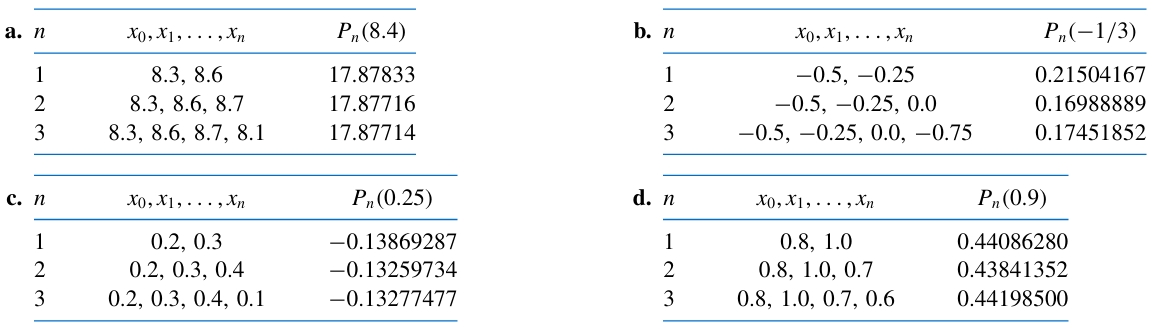
\includegraphics[width=15cm]{CompQuizMod3Sec1}
\end{center}
\end{mysolution}
\end{myexercise}

\section{Divided Differences}

\begin{youtube}
This videos presents a discussion on divided differences. Follow the discussion and then solve the problems in the subsequent quiz.

\end{youtube}
\mylink{https://www.youtube.com/watch?\\v=BAwOGkchq7w\&list=PLDea8VeK4MUTppAXQzHBNz3KiyEd9SQms\&index=66}

\mylink{https://www.youtube.com/watch?\\v=A8rFozfIWmg\&list=PLDea8VeK4MUTppAXQzHBNz3KiyEd9SQms\&index=67}

\mylink{https://www.youtube.com/watch?v=h-\\MO4BnQWHs\&list=PLDea8VeK4MUTppAXQzHBNz3KiyEd9SQms\&index=68}

\mylink{https://www.youtube.com/watch?v=xVA-\\C1hHu1o\&list=PLDea8VeK4MUTppAXQzHBNz3KiyEd9SQms\&index=69}

\begin{myexercise}%\label{Comprehensionquiz2}
Use 
\[P_n(x)=f[x_0]+\sum^n_{k=1}f[x_0, x_1, \ldots, x_k](x-x_0)\cdots(x-x_{k-1})\]
to construct interpolating polynomials of degree one, two, and three for the following data. Approximate the specified value using each of the polynomials.
\begin{enumerate}[label=(\alph*)]
\item $f(8.4)$ if $f(8.1)=16.94410$, $f(8.3)=17.56492$, $f(8.6)=18.50515$, $f(8.7)=18.82091$
\item $f(0.9)$ if $f(0.6)=-0.17694460$, $f(0.7)=0.01375227$, $f(0.8)=0.22363362$, $f(1.0)=0.65809197$
\end{enumerate}
\begin{mysolution}
\begin{enumerate}[label=(\alph*)]
\item $P_1(x) = 16.9441 +3.1041(x -8.1)$; $P_1(8.4) = 17.87533$, $P_2(x) = P_1(x) + 0.06(x - 8.1)(x - 8.3)$; $P_2(8.4) = 17.87713$, $P_3(x) = P_2(x)-0.00208333(x- 8.1)(x - 8.3)(x-8.6)$; $P_3(8.4) = 17.87714$
\item $P_1(x) =-0.1769446 +1.9069687(x-0.6)$; $P1(0.9) = 0.395146$, $P_2(x) = P_1(x) +0.959224(x-0.6)(x-0.7)$; $P_2(0.9) = 0.4526995$, $P_3(x) = P_2(x)-1.785741(x-0.6)(x-0.7)(x-0.8)$; $P_3(0.9) = 0.4419850$
\end{enumerate}
\end{mysolution}
\end{myexercise}



\section{Hermite Interpolation}
\videolesson
\begin{selfvideo}[2]
%LESSON 3: 
This video presents a discussion on Hermite interpolation. Follow the discussion and then solve the problems in the subsequent quiz.
\end{selfvideo}
%\activities
%Read on Hermite interpolation in pages \textcolor{red}{\bf page $136-142$} of the following reference and then attempt the subsequent quiz
%\begin{activity}[\cg Reading]
%\begin{enumerate}
%\item Burden, R. L., Faires, J. D., Burden, A. M. (2015). Numerical Analysis. Tenth Edition, Cengage Learning.\\
%\end{enumerate}
%\end{activity}


\begin{definition}
 Let $x_0, x_1, \ldots, x_n$ be $n + 1$ distinct numbers in $[a,b]$ and for $i = 0, 1, \ldots, n$ let $m_i$ be a  nonnegative integer. Suppose that $f\in C^m[a,b]$, where $m =\max_{0\leq i\leq n} m_i$. The {\bf osculating polynomial} approximating $f$ is the polynomial $P(x)$ of least degree such that
\[\frac{d^kP(x_i)}{dx^k}=\frac{d^kf(x_i)}{dx^k},\quad\mbox{for each} i = 0, 1, \ldots, n\quad \mbox{and}\quad k = 0, 1, \ldots, m_i.\]
\end{definition}

Note that when $n = 0$, the osculating polynomial approximating $f$ is the $m_0$th Taylor polynomial for $f$ at $x_0$. When $m_i = 0$ for each $i$, the osculating polynomial is the $n$th Lagrange polynomial interpolating $f$ on $x_0, x_1, \ldots, x_n$

\subsection*{ Hermite Polynomials}\label{thm:hermite1}
The case when $m_i = 1$, for each $i = 0, 1, \ldots, n$, gives the {\bf Hermite polynomials}. For a given function $f$, these polynomials agree with $f$ at $x_0, x_1, \ldots, x_n$. In addition, since their first derivatives agree with those of $f$, they have the same ``shape'' as the function at $(x_i, f(x_i))$ in the sense that the tangent lines to the polynomial and the function agree. We will restrict our study of osculating polynomials to this situation and consider first a theorem that describes precisely the form of the Hermite polynomials.

\begin{theorem}\label{Hermitthm1}
If $f \in C^{1}[a, b]$ and $x_{0}, \ldots, x_{n} \in[a, b]$ are distinct, the unique polynomial of least degree agreeing with $f$ and $f^{\prime}$ at $x_{0}, \ldots, x_{n}$ is the Hermite polynomial of degree at most $2 n+1$ given by

$$
H_{2 n+1}(x)=\sum_{j=0}^{n} f\left(x_{j}\right) H_{n, j}(x)+\sum_{j=0}^{n} f^{\prime}\left(x_{j}\right) \hat{H}_{n, j}(x),
$$

%Hermite gave a description of a general osculatory polynomial in a letter to Carl W. Borchardt in 1878, to whom he regularly sent his new results. His demonstration is an interesting application of the use of complex integration techniques to solve a real-valued problem.\\
where, for $L_{n, j}(x)$ denoting the $j$ th Lagrange coefficient polynomial of degree $n$, we have

$$
H_{n, j}(x)=\left[1-2\left(x-x_{j}\right) L_{n, j}^{\prime}\left(x_{j}\right)\right] L_{n, j}^{2}(x) \quad \text { and } \quad \hat{H}_{n, j}(x)=\left(x-x_{j}\right) L_{n, j}^{2}(x) .
$$

Moreover, if $f \in C^{2 n+2}[a, b]$, then

$$
f(x)=H_{2 n+1}(x)+\frac{\left(x-x_{0}\right)^{2} \ldots\left(x-x_{n}\right)^{2}}{(2 n+2)!} f^{(2 n+2)}(\xi(x)),
$$

for some (generally unknown) $\xi(x)$ in the interval $(a, b)$.
\end{theorem}

%Proof First recall that
%
%$$
%L_{n, j}\left(x_{i}\right)= \begin{cases}0, & \text { if } i \neq j \\ 1, & \text { if } i=j\end{cases}
%$$
%
%Hence when $i \neq j$,
%
%$$
%H_{n, j}\left(x_{i}\right)=0 \quad \text { and } \quad \hat{H}_{n, j}\left(x_{i}\right)=0,
%$$
%
%whereas, for each $i$,
%
%$$
%H_{n, i}\left(x_{i}\right)=\left[1-2\left(x_{i}-x_{i}\right) L_{n, i}^{\prime}\left(x_{i}\right)\right] \cdot 1=1 \quad \text { and } \quad \hat{H}_{n, i}\left(x_{i}\right)=\left(x_{i}-x_{i}\right) \cdot 1^{2}=0 .
%$$
%
%As a consequence
%
%$$
%H_{2 n+1}\left(x_{i}\right)=\sum_{\substack{j=0 \\ j \neq i}}^{n} f\left(x_{j}\right) \cdot 0+f\left(x_{i}\right) \cdot 1+\sum_{j=0}^{n} f^{\prime}\left(x_{j}\right) \cdot 0=f\left(x_{i}\right),
%$$
%
%so $H_{2 n+1}$ agrees with $f$ at $x_{0}, x_{1}, \ldots, x_{n}$.\\
%To show the agreement of $H_{2 n+1}^{\prime}$ with $f^{\prime}$ at the nodes, first note that $L_{n, j}(x)$ is a factor of $H_{n, j}^{\prime}(x)$, so $H_{n, j}^{\prime}\left(x_{i}\right)=0$ when $i \neq j$. In addition, when $i=j$ we have $L_{n, i}\left(x_{i}\right)=1$, so
%
%$$
%\begin{aligned}
%H_{n, i}^{\prime}\left(x_{i}\right) & =-2 L_{n, i}^{\prime}\left(x_{i}\right) \cdot L_{n, i}^{2}\left(x_{i}\right)+\left[1-2\left(x_{i}-x_{i}\right) L_{n, i}^{\prime}\left(x_{i}\right)\right] 2 L_{n, i}\left(x_{i}\right) L_{n, i}^{\prime}\left(x_{i}\right) \\
%& =-2 L_{n, i}^{\prime}\left(x_{i}\right)+2 L_{n, i}^{\prime}\left(x_{i}\right)=0
%\end{aligned}
%$$
%
%Hence, $H_{n, j}^{\prime}\left(x_{i}\right)=0$ for all $i$ and $j$.\\
%Finally,
%
%$$
%\begin{aligned}
%\hat{H}_{n, j}^{\prime}\left(x_{i}\right) & =L_{n, j}^{2}\left(x_{i}\right)+\left(x_{i}-x_{j}\right) 2 L_{n, j}\left(x_{i}\right) L_{n, j}^{\prime}\left(x_{i}\right) \\
%& =L_{n, j}\left(x_{i}\right)\left[L_{n, j}\left(x_{i}\right)+2\left(x_{i}-x_{j}\right) L_{n, j}^{\prime}\left(x_{i}\right)\right],
%\end{aligned}
%$$
%
%so $\hat{H}_{n, j}^{\prime}\left(x_{i}\right)=0$ if $i \neq j$ and $\hat{H}_{n, i}^{\prime}\left(x_{i}\right)=1$. Combining these facts, we have
%
%$$
%H_{2 n+1}^{\prime}\left(x_{i}\right)=\sum_{j=0}^{n} f\left(x_{j}\right) \cdot 0+\sum_{\substack{j=0 \\ j \neq i}}^{n} f^{\prime}\left(x_{j}\right) \cdot 0+f^{\prime}\left(x_{i}\right) \cdot 1=f^{\prime}\left(x_{i}\right) .
%$$
%
%Therefore, $H_{2 n+1}$ agrees with $f$ and $H_{2 n+1}^{\prime}$ with $f^{\prime}$ at $x_{0}, x_{1}, \ldots, x_{n}$.\\
%The uniqueness of this polynomial and the error formula are considered in Exercise 11.
%
\begin{example}\label{exam:hermite1}
Use the Hermite polynomial that agrees with the data listed in Table \ref{tab:hermiteexample1} to find an approximation of $f(1.5)$.
\end{example}
%Table 3.15

\begin{table}
\centering
\begin{tabular}{cccc}
\hline
$k$ & $x_{k}$ & $f\left(x_{k}\right)$ & $f^{\prime}\left(x_{k}\right)$ \\
\hline
0 & 1.3 & 0.6200860 & -0.5220232 \\
1 & 1.6 & 0.4554022 & -0.5698959 \\
2 & 1.9 & 0.2818186 & -0.5811571 \\
\hline
\end{tabular}
\caption{\scriptsize Table $8$}
\label{tab:hermiteexample1}
\end{table}

\begin{mysolution}
We first compute the Lagrange polynomials and their derivatives. This gives

$$
\begin{aligned}
& L_{2,0}(x)=\frac{\left(x-x_{1}\right)\left(x-x_{2}\right)}{\left(x_{0}-x_{1}\right)\left(x_{0}-x_{2}\right)}=\frac{50}{9} x^{2}-\frac{175}{9} x+\frac{152}{9}, \quad L_{2,0}^{\prime}(x)=\frac{100}{9} x-\frac{175}{9} ; \\
& L_{2,1}(x)=\frac{\left(x-x_{0}\right)\left(x-x_{2}\right)}{\left(x_{1}-x_{0}\right)\left(x_{1}-x_{2}\right)}=\frac{-100}{9} x^{2}+\frac{320}{9} x-\frac{247}{9}, \quad L_{2,1}^{\prime}(x)=\frac{-200}{9} x+\frac{320}{9} ;
\end{aligned}
$$

and

$$
L_{2,2}=\frac{\left(x-x_{0}\right)\left(x-x_{1}\right)}{\left(x_{2}-x_{0}\right)\left(x_{2}-x_{1}\right)}=\frac{50}{9} x^{2}-\frac{145}{9} x+\frac{104}{9}, \quad \quad L_{2,2}^{\prime}(x)=\frac{100}{9} x-\frac{145}{9} .
$$

The polynomials $H_{2, j}(x)$ and $\hat{H}_{2, j}(x)$ are then

$$
\begin{aligned}
H_{2,0}(x) & =[1-2(x-1.3)(-5)]\left(\frac{50}{9} x^{2}-\frac{175}{9} x+\frac{152}{9}\right)^{2} \\
& =(10 x-12)\left(\frac{50}{9} x^{2}-\frac{175}{9} x+\frac{152}{9}\right)^{2} \\
H_{2,1}(x) & =1 \cdot\left(\frac{-100}{9} x^{2}+\frac{320}{9} x-\frac{247}{9}\right)^{2} \\
H_{2,2}(x) & =10(2-x)\left(\frac{50}{9} x^{2}-\frac{145}{9} x+\frac{104}{9}\right)^{2} \\
\hat{H}_{2,0}(x) & =(x-1.3)\left(\frac{50}{9} x^{2}-\frac{175}{9} x+\frac{152}{9}\right)^{2} \\
\hat{H}_{2,1}(x) & =(x-1.6)\left(\frac{-100}{9} x^{2}+\frac{320}{9} x-\frac{247}{9}\right)^{2}
\end{aligned}
$$

and

$$
\hat{H}_{2,2}(x)=(x-1.9)\left(\frac{50}{9} x^{2}-\frac{145}{9} x+\frac{104}{9}\right)^{2}
$$

Finally

$$
\begin{aligned}
H_{5}(x)= & 0.6200860 H_{2,0}(x)+0.4554022 H_{2,1}(x)+0.2818186 H_{2,2}(x) \\
& -0.5220232 \hat{H}_{2,0}(x)-0.5698959 \hat{H}_{2,1}(x)-0.5811571 \hat{H}_{2,2}(x)
\end{aligned}
$$

and

$$
\begin{aligned}
H_{5}(1.5)= & 0.6200860\left(\frac{4}{27}\right)+0.4554022\left(\frac{64}{81}\right)+0.2818186\left(\frac{5}{81}\right) \\
& -0.5220232\left(\frac{4}{405}\right)-0.5698959\left(\frac{-32}{405}\right)-0.5811571\left(\frac{-2}{405}\right) \\
= & 0.5118277
\end{aligned}
$$

a result that is accurate to the places listed.
\end{mysolution}

Although Theorem \ref{thm:hermite1} provides a complete description of the Hermite polynomials, it is clear from Example \ref{exam:hermite1} that the need to determine and evaluate the Lagrange polynomials and their derivatives makes the procedure tedious even for small values of $n$.

\subsection*{Hermite Polynomials Using Divided Differences}
There is an alternative method for generating Hermite approximations that has as its basis the Newton interpolatory divided-difference formula at $x_{0}, x_{1}, \ldots, x_{n}$, given by

$$
P_{n}(x)=f\left[x_{0}\right]+\sum_{k=1}^{n} f\left[x_{0}, x_{1}, \ldots, x_{k}\right]\left(x-x_{0}\right) \cdots\left(x-x_{k-1}\right)
$$
The alternative method uses the connection between the $n$th divided difference and the $n$th derivative of $f$.

Suppose that the distinct numbers $x_{0}, x_{1}, \ldots, x_{n}$ are given together with the values of $f$ and $f^{\prime}$ at these numbers. Define a new sequence $z_{0}, z_{1}, \ldots, z_{2 n+1}$ by

$$
z_{2 i}=z_{2 i+1}=x_{i}, \quad \text { for each } i=0,1, \ldots, n,
$$
and construct the divided difference table in the form of Table 3.9 that uses $z_{0}, z_{1}, \ldots, z_{2 n+1}$.

Since $z_{2 i}=z_{2 i+1}=x_{i}$ for each $i$, we cannot define $f\left[z_{2 i}, z_{2 i+1}\right]$ by the divided difference formula. However, if we assume, based on Theorem 3.6, that the reasonable substitution in this situation is $f\left[z_{2 i}, z_{2 i+1}\right]=f^{\prime}\left(z_{2 i}\right)=f^{\prime}\left(x_{i}\right)$, we can use the entries

$$
f^{\prime}\left(x_{0}\right), f^{\prime}\left(x_{1}\right), \ldots, f^{\prime}\left(x_{n}\right)
$$
in place of the undefined first divided differences

$$
f\left[z_{0}, z_{1}\right], f\left[z_{2}, z_{3}\right], \ldots, f\left[z_{2 n}, z_{2 n+1}\right] .
$$

The remaining divided differences are produced as usual, and the appropriate divided differences are employed in Newton's interpolatory divided-difference formula. Table \ref{tab:hermite2} shows the entries that are used for the first three divided-difference columns when determining the Hermite polynomial $H_{5}(x)$ for $x_{0}, x_{1}$, and $x_{2}$. The remaining entries are generated in the same manner as in Table \ref{tab:hermite2}. The Hermite polynomial is then given by

$$
H_{2 n+1}(x)=f\left[z_{0}\right]+\sum_{k=1}^{2 n+1} f\left[z_{0}, \ldots, z_{k}\right]\left(x-z_{0}\right)\left(x-z_{1}\right) \cdots\left(x-z_{k-1}\right)
$$

%A proof of this fact can be found in [Pow], p. 56.
%
%Table 3.16

\begin{table}
\centering
\begin{tabular}{|l|l|l|l|}
\hline
$z$ & $f(z)$ & First divided differences & Second divided differences \\
\hline
$z_{0}=x_{0}$ & $f\left[z_{0}\right]=f\left(x_{0}\right)$ &  &  \\
\hline
 &  & $f\left[z_{0}, z_{1}\right]=f^{\prime}\left(x_{0}\right)$ &  \\
\hline
$z_{1}=x_{0}$ & $f\left[z_{1}\right]=f\left(x_{0}\right)$ &  & $f\left[z_{0}, z_{1}, z_{2}\right]=\frac{f\left[z_{1}, z_{2}\right]-f\left[z_{0}, z_{1}\right]}{z_{2}-z_{0}}$ \\
\hline
 &  & $f\left[z_{1}, z_{2}\right]=\frac{f\left[z_{2}\right]-f\left[z_{1}\right]}{z_{2}-z_{1}}$ &  \\
\hline
$z_{2}=x_{1}$ & $f\left[z_{2}\right]=f\left(x_{1}\right)$ &  & $f\left[z_{1}, z_{2}, z_{3}\right]=\frac{f\left[z_{2}, z_{3}\right]-f\left[z_{1}, z_{2}\right]}{z_{3}-z_{1}}$ \\
\hline
 &  & $f\left[z_{2}, z_{3}\right]=f^{\prime}\left(x_{1}\right)$ &  \\
\hline
$z_{3}=x_{1}$ & $f\left[z_{3}\right]=f\left(x_{1}\right)$ &  & $f\left[z_{2}, z_{3}, z_{4}\right]=\frac{f\left[z_{3}, z_{4}\right]-f\left[z_{2}, z_{3}\right]}{z_{4}-z_{2}}$ \\
\hline
 &  & $f\left[z_{3}, z_{4}\right]=\frac{f\left[z_{4}\right]-f\left[z_{3}\right]}{z_{4}-z_{3}}$ &  \\
\hline
$z_{4}=x_{2}$ & $f\left[z_{4}\right]=f\left(x_{2}\right)$ &  & $f\left[z_{3}, z_{4}, z_{5}\right]=\frac{f\left[z_{4}, z_{5}\right]-f\left[z_{3}, z_{4}\right]}{z_{5}-z_{3}}$ \\
\hline
 &  & $f\left[z_{4}, z_{5}\right]=f^{\prime}\left(x_{2}\right)$ &  \\
\hline
$z_{5}=x_{2}$ & $f\left[z_{5}\right]=f\left(x_{2}\right)$ &  &  \\
\hline
\end{tabular}
\caption{\scriptsize Table $9$}
\label{tab:hermite2}
\end{table}

\begin{example}
Use the data given in Example 1 and the divided difference method to determine the Hermite polynomial approximation at $x=1.5$.
\end{example}

\begin{mysolution}The underlined entries in the first three columns of Table \ref{tab:hermiteexample2} are the data given in Example \ref{exam:hermite1}. The remaining entries in this table are generated by the standard divided difference formula relative to $x_i, x_{i+1}, \ldots, x_{i+k}$ given by
\[f[x_i, x_{i+1}, \ldots, x_{i+k}]=\frac{f[x_i, x_{i+1}, \ldots, x_{i+k}]-f[x_1, x_{i+1}, \ldots, x_{i+k-1}]}{x_{i+k}-x_1}\]

For example, for the second entry in the third column we use the second $1.3$ entry in the second column and the first $1.6$ entry in that column to obtain

$$
\frac{0.4554022-0.6200860}{1.6-1.3}=-0.5489460 .
$$
For the first entry in the fourth column we use the first $1.3$ entry in the third column and the first $1.6$ entry in that column to obtain

$$
\frac{-0.5489460-(-0.5220232)}{1.6-1.3}=-0.0897427 .
$$
The value of the Hermite polynomial at $1.5$ is

$$
\begin{aligned}
H_{5}(1.5)= & f[1.3]+f^{\prime}(1.3)(1.5-1.3)+f[1.3,1.3,1.6](1.5-1.3)^{2} \\
& +f[1.3,1.3,1.6,1.6](1.5-1.3)^{2}(1.5-1.6) \\
& +f[1.3,1.3,1.6,1.6,1.9](1.5-1.3)^{2}(1.5-1.6)^{2} \\
& +f[1.3,1.3,1.6,1.6,1.9,1.9](1.5-1.3)^{2}(1.5-1.6)^{2}(1.5-1.9) \\
= & 0.6200860+(-0.5220232)(0.2)+(-0.0897427)(0.2)^{2} \\
& +0.0663657(0.2)^{2}(-0.1)+0.0026663(0.2)^{2}(-0.1)^{2} \\
& +(-0.0027738)(0.2)^{2}(-0.1)^{2}(-0.4) \\
= & 0.5118277
\end{aligned}
$$
\end{mysolution}
%Table 3.17
%
\begin{table}
\centering
\begin{tabular}{|l|l|l|l|l|l|l|}
\hline
1.3 & 0.6200860 & \multicolumn{5}{|c|}{} \\
\hline
 &  & -0.5220232 &  & \multirow[b]{3}{*}{0.0663657} & \multirow{3}{*}{} & \multirow{3}{*}{} \\
\hline
$\underline{1.3}$ & 0.6200860 &  & -0.0897427 &  &  &  \\
\hline
 &  & -0.5489460 & \multirow[b]{2}{*}{-0.0698330} &  &  &  \\
\hline
1.6 & 0.4554022 &  &  & \multicolumn{3}{|c|}{0.0026663} \\
\hline
\multicolumn{2}{|c|}{} & -0.5698959 & \multirow[b]{2}{*}{-0.0290537} & 0.0679655 & \multicolumn{2}{|r|}{-0.0027738} \\
\hline
1.6 & 0.4554022 & \multirow[b]{2}{*}{-0.5786120} &  &  & 0.0010020 &  \\
\hline
\multicolumn{2}{|c|}{} &  &  & 0.0685667 &  &  \\
\hline
1.9 & 0.2818186 & \multirow[b]{2}{*}{-0.5811571} & -0.0084837 &  &  &  \\
\hline
\multicolumn{2}{|c|}{} &  &  &  &  &  \\
\hline
1.9 & 0.2818186 &  &  &  &  &  \\
\hline
\end{tabular}
\caption{\scriptsize Table $10$}
\label{tab:hermiteexample2}
\end{table}


\begin{myexercise}%\label{Comprehensionquiz2}
Use Theorem \ref{Hermitthm1} to construct an approximating polynomial for the following data.
\begin{enumerate}[label=(\alph*)]
\item
\begin{center}
\begin{tabular}{c|c|c}
$x$ & $f(x)$ & $f^{\prime}(x)$ \\
\hline
8.3 & 17.56492 & 3.116256 \\
8.6 & 18.50515 & 3.151762 \\
\end{tabular}
\end{center}

\item
\begin{center}
\begin{tabular}{c|c|c}
$x$ & $f(x)$ & $f^{\prime}(x)$ \\
\hline
0.8 & 0.22363362 & 2.1691753 \\
1.0 & 0.65809197 & 2.0466965 \\
\end{tabular}
\end{center}

\item
\begin{center}
\begin{tabular}{l|r|c}
\multicolumn{1}{c|}{$x$} & \multicolumn{1}{c|}{$f(x)$} & $f^{\prime}(x)$ \\
\hline
-0.5 & -0.0247500 & 0.7510000 \\
-0.25 & 0.3349375 & 2.1890000 \\
0 & 1.1010000 & 4.0020000 \\
\end{tabular}
\end{center}

\item
\begin{center}
\begin{tabular}{c|r|c}
$x$ & \multicolumn{1}{|c|}{$f(x)$} & \multicolumn{1}{c}{$f^{\prime}(x)$} \\
\hline
0.1 & -0.62049958 & 3.58502082 \\
0.2 & -0.28398668 & 3.14033271 \\
0.3 & 0.00660095 & 2.66668043 \\
0.4 & 0.24842440 & 2.16529366 \\
\end{tabular}
\end{center}
\end{enumerate}

\begin{mysolution}
The coefficients for the polynomials in divided-difference form are given in the following tables. For example, the polynomial in part (a) is
\[\begin{split}
H_3(x)=&17.56492+3.116256(x-8.3)+0.05948(x-8.3)^2-\\
&0.00202222(x-8.3)^2(x-8.6).
\end{split}\]
\begin{center}
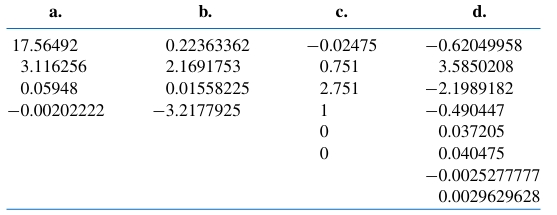
\includegraphics[width=12cm]{CompQuizMod3Sec3Sol}
\end{center}
\end{mysolution}
\end{myexercise}

\section{Cubic Spline Interpolation}
\begin{youtube}
This video presents a discussion on cubic spline interpolation. Follow the discussion and then solve the problems in the subsequent quiz.
\end{youtube}

\mylink{https://www.youtube.com/watch?\\v=pBtqaK0PzrA\&list=PLDea8VeK4MUTppAXQzHBNz3KiyEd9SQms\&index=77}

\mylink{https://www.youtube.com/watch?\\v=yOUst2672qo\&list=PLDea8VeK4MUTppAXQzHBNz3KiyEd9SQms\&index=78}

\mylink{https://www.youtube.com/watch?\\v=\_6\_z7DzDhUo\&list=PLDea8VeK4MUTppAXQzHBNz3KiyEd9SQms\&index=79}

%\videolesson
%\begin{selfvideo}[2]
%%LESSON 3: 
%This video presents a discussion on cubic spline interpolation. Follow the discussion and then solve the problems in the subsequent quiz.
%\end{selfvideo}
%\begin{boxB}Question: \end{boxB}
%The previous sections concerned the approximation of arbitrary functions on closed intervals using a single polynomial. However, high-degree polynomials can oscillate erratically, that is, a minor fluctuation over a small portion of the interval can induce large fluctuations over the entire range. 
%
%An alternative approach is to divide the approximation interval into a collection of subintervals and construct a (generally) different approximating polynomial on each subinterval. This is called {\bf piecewise-polynomial approximation}.
%
%\subsection*{Piecewise-Polynomial Approximation}
%The simplest piecewise-polynomial approximation is {\bf piecewise-linear} interpolation, which consists of joining a set of data points
%\[\left\{\left(x_{0}, f\left(x_{0}\right)\right),\left(x_{1}, f\left(x_{1}\right)\right), \ldots,\left(x_{n}, f\left(x_{n}\right)\right)\right\}\]
%by a series of straight lines, as shown in Figure \ref{fig:piecewiselinapproxpic1}
%\begin{figure}[h]
%\centering
%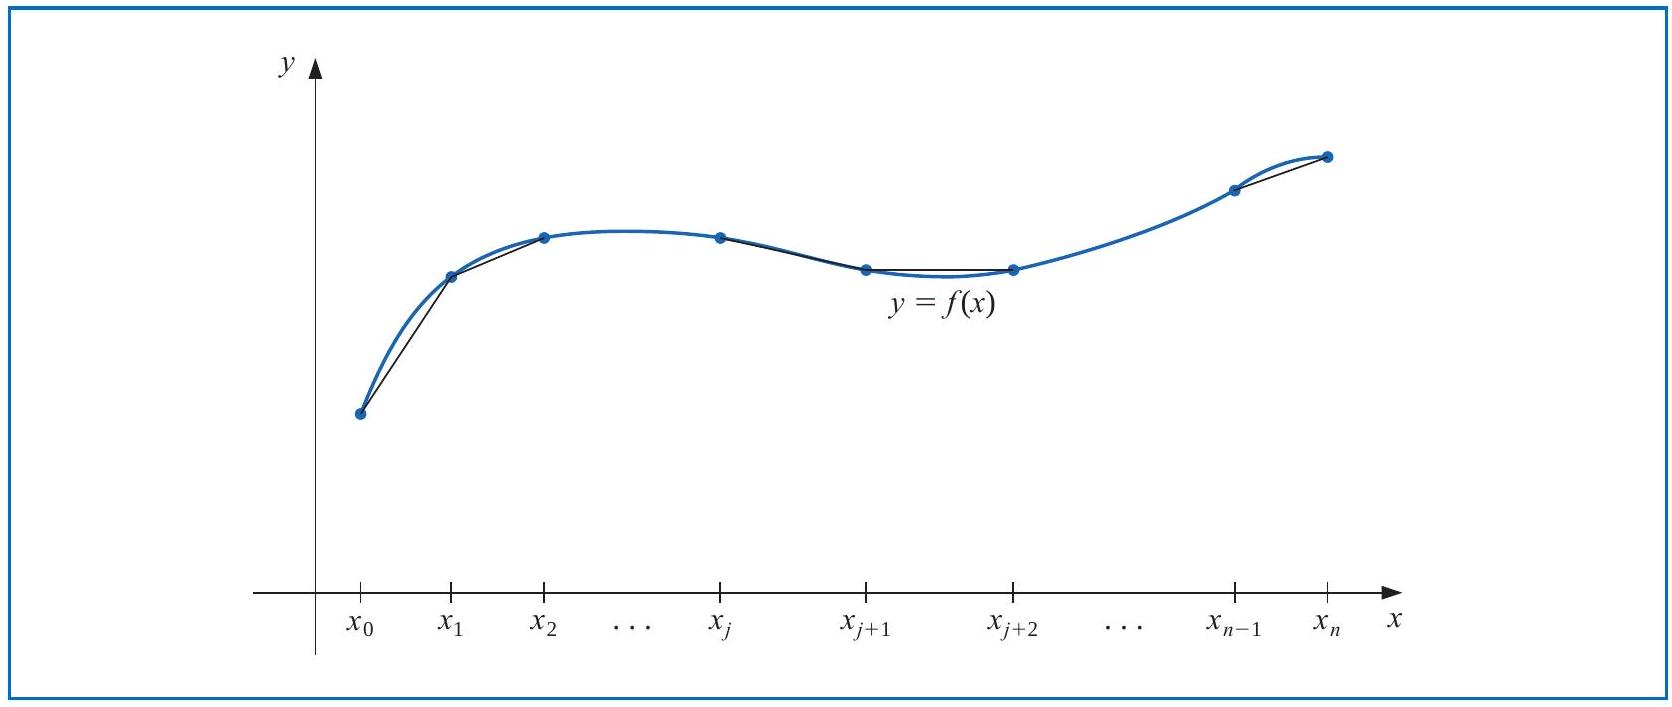
\includegraphics[width=9cm]{piecewiselinapproxpic1.JPG}
%\caption{}
%\label{fig:piecewiselinapproxpic1}
%\end{figure}
%
%A disadvantage of linear function approximation is that there is likely no differentiability at the endpoints of the subintervals, which, in a geometrical context, means that the interpolating function is not "smooth." Often it is clear from physical conditions that smoothness is required, so the approximating function must be continuously differentiable.
%
%An alternative procedure is to use a piecewise polynomial of Hermite type. For example, if the values of $f$ and of $f^{\prime}$ are known at each of the points $x_{0}<x_{1}<\cdots<x_{n}$, a cubic Hermite polynomial can be used on each of the subintervals $\left[x_{0}, x_{1}\right],\left[x_{1}, x_{2}\right], \ldots,\left[x_{n-1}, x_{n}\right]$ to obtain a function that has a continuous derivative on the interval $\left[x_{0}, x_{n}\right]$.\\
%${ }^{1}$.
%%
%%Figure 3.7\\
%
%%
%%Isaac Jacob Schoenberg (1903-1990) developed his work on splines during World War II while on leave from the University of Pennsylvania to work at the Army's Ballistic\\
%%Research Laboratory in Aberdeen, Maryland. His original work involved numerical procedures for solving differential equations. The much broader application of splines to the areas of data fitting and computer-aided geometric design became evident with the widespread availability of computers in the 1960s.
%
%To determine the appropriate Hermite cubic polynomial on a given interval is simply a matter of computing $H_{3}(x)$ for that interval. The Lagrange interpolating polynomials needed to determine $H_{3}$ are of first degree, so this can be accomplished without great difficulty. However, to use Hermite piecewise polynomials for general interpolation, we need to know the derivative of the function being approximated, and this is frequently unavailable.
%
%The remainder of this section considers approximation using piecewise polynomials that require no specific derivative information, except perhaps at the endpoints of the interval on which the function is being approximated.
%
%The simplest type of differentiable piecewise-polynomial function on an entire interval $\left[x_{0}, x_{n}\right]$ is the function obtained by fitting one quadratic polynomial between each successive pair of nodes. This is done by constructing a quadratic on $\left[x_{0}, x_{1}\right]$ agreeing with the function at $x_{0}$ and $x_{1}$, another quadratic on $\left[x_{1}, x_{2}\right]$ agreeing with the function at $x_{1}$ and $x_{2}$, and so on. A general quadratic polynomial has three arbitrary constants-the constant term, the coefficient of $x$, and the coefficient of $x^{2}$-and only two conditions are required to fit the data at the endpoints of each subinterval. So flexibility exists that permits the quadratics to be chosen so that the interpolant has a continuous derivative on $\left[x_{0}, x_{n}\right]$. The difficulty arises because we generally need to specify conditions about the derivative of the interpolant at the endpoints $x_{0}$ and $x_{n}$. There is not a sufficient number of constants to ensure that the conditions will be satisfied.
%
%\subsection*{Cubic Splines}
%The most common piecewise-polynomial approximation uses cubic polynomials between each successive pair of nodes and is called {\bf cubic spline interpolation}. A general cubic polynomial involves four constants, so there is sufficient flexibility in the cubic spline procedure to ensure that the interpolant is not only continuously differentiable on the interval, but also has a continuous second derivative. The construction of the cubic spline does not, however, assume that the derivatives of the interpolant agree with those of the function it is approximating, even at the nodes. (See Figure 3.8.)
%
%Figure 3.8\\
%\includegraphics[max width=\textwidth, center]{2025_05_15_4109a88b43049bd640d1g-42(1)}
%
%Definition 3.10
%
%A natural spline has no conditions imposed for the direction at its endpoints, so the curve takes the shape of a straight line after it passes through the interpolation points nearest its endpoints. The name derives from the fact that this is the natural shape a flexible strip assumes if forced to pass through specified interpolation points with no additional constraints. (See Figure 3.9.)\\
%\includegraphics[max width=\textwidth, center]{2025_05_15_4109a88b43049bd640d1g-42}
%
%Figure 3.9
%
%Given a function $f$ defined on $[a, b]$ and a set of nodes $a=x_{0}<x_{1}<\cdots<$ $x_{n}=b$, a cubic spline interpolant $S$ for $f$ is a function that satisfies the following conditions:\\
%(a) $\quad S(x)$ is a cubic polynomial, denoted $S_{j}(x)$, on the subinterval $\left[x_{j}, x_{j+1}\right]$ for each $j=0,1, \ldots, n-1 ;$\\
%(b) $\quad S_{j}\left(x_{j}\right)=f\left(x_{j}\right)$ and $S_{j}\left(x_{j+1}\right)=f\left(x_{j+1}\right)$ for each $j=0,1, \ldots, n-1$;\\
%(c) $S_{j+1}\left(x_{j+1}\right)=S_{j}\left(x_{j+1}\right)$ for each $j=0,1, \ldots, n-2$; (Implied by (b).)\\
%(d) $\quad S_{j+1}^{\prime}\left(x_{j+1}\right)=S_{j}^{\prime}\left(x_{j+1}\right)$ for each $j=0,1, \ldots, n-2$;\\
%(e) $S_{j+1}^{\prime \prime}\left(x_{j+1}\right)=S_{j}^{\prime \prime}\left(x_{j+1}\right)$ for each $j=0,1, \ldots, n-2$;\\
%(f) One of the following sets of boundary conditions is satisfied:\\
%(i) $\quad S^{\prime \prime}\left(x_{0}\right)=S^{\prime \prime}\left(x_{n}\right)=0 \quad$ (natural (or free) boundary);\\
%(ii) $\quad S^{\prime}\left(x_{0}\right)=f^{\prime}\left(x_{0}\right)$ and $\quad S^{\prime}\left(x_{n}\right)=f^{\prime}\left(x_{n}\right) \quad$ (clamped boundary).
%
%Although cubic splines are defined with other boundary conditions, the conditions given in (f) are sufficient for our purposes. When the free boundary conditions occur, the spline is called a natural spline, and its graph approximates the shape that a long flexible rod would assume if forced to go through the data points $\left\{\left(x_{0}, f\left(x_{0}\right)\right),\left(x_{1}, f\left(x_{1}\right)\right), \ldots,\left(x_{n}, f\left(x_{n}\right)\right)\right\}$.
%
%In general, clamped boundary conditions lead to more accurate approximations because they include more information about the function. However, for this type of boundary condition to hold, it is necessary to have either the values of the derivative at the endpoints or an accurate approximation to those values.
%
%Example 1 Construct a natural cubic spline that passes through the points $(1,2),(2,3)$, and $(3,5)$.\\[0pt]
%Solution This spline consists of two cubics. The first for the interval [1, 2], denoted
%
%$$
%S_{0}(x)=a_{0}+b_{0}(x-1)+c_{0}(x-1)^{2}+d_{0}(x-1)^{3},
%$$
%
%Clamping a spline indicates that the ends of the flexible strip are fixed so that it is forced to take a specific direction at each of its endpoints. This is important, for example, when two spline functions should match at their endpoints. This is done mathematically by specifying the values of the derivative of the curve at the endpoints of the spline.\\[0pt]
%and the other for [2,3], denoted
%
%$$
%S_{1}(x)=a_{1}+b_{1}(x-2)+c_{1}(x-2)^{2}+d_{1}(x-2)^{3} .
%$$
%
%There are 8 constants to be determined, which requires 8 conditions. Four conditions come from the fact that the splines must agree with the data at the nodes. Hence
%
%$$
%\begin{aligned}
%& 2=f(1)=a_{0}, \quad 3=f(2)=a_{0}+b_{0}+c_{0}+d_{0}, \quad 3=f(2)=a_{1}, \quad \text { and } \\
%& 5=f(3)=a_{1}+b_{1}+c_{1}+d_{1} .
%\end{aligned}
%$$
%
%Two more come from the fact that $S_{0}^{\prime}(2)=S_{1}^{\prime}(2)$ and $S_{0}^{\prime \prime}(2)=S_{1}^{\prime \prime}(2)$. These are
%
%$$
%S_{0}^{\prime}(2)=S_{1}^{\prime}(2): \quad b_{0}+2 c_{0}+3 d_{0}=b_{1} \quad \text { and } \quad S_{0}^{\prime \prime}(2)=S_{1}^{\prime \prime}(2): \quad 2 c_{0}+6 d_{0}=2 c_{1}
%$$
%
%The final two come from the natural boundary conditions:
%
%$$
%S_{0}^{\prime \prime}(1)=0: \quad 2 c_{0}=0 \quad \text { and } \quad S_{1}^{\prime \prime}(3)=0: \quad 2 c_{1}+6 d_{1}=0 .
%$$
%
%Solving this system of equations gives the spline
%
%$$
%S(x)=\left\{\begin{array}{l}
%2+\frac{3}{4}(x-1)+\frac{1}{4}(x-1)^{3}, \text { for } x \in[1,2] \\
%3+\frac{3}{2}(x-2)+\frac{3}{4}(x-2)^{2}-\frac{1}{4}(x-2)^{3}, \text { for } x \in[2,3]
%\end{array}\right.
%$$
%
%\section*{Construction of a Cubic Spline}
%As the preceding example demonstrates, a spline defined on an interval that is divided into $n$ subintervals will require determining $4 n$ constants. To construct the cubic spline interpolant for a given function $f$, the conditions in the definition are applied to the cubic polynomials
%
%$$
%S_{j}(x)=a_{j}+b_{j}\left(x-x_{j}\right)+c_{j}\left(x-x_{j}\right)^{2}+d_{j}\left(x-x_{j}\right)^{3},
%$$
%
%for each $j=0,1, \ldots, n-1$. Since $S_{j}\left(x_{j}\right)=a_{j}=f\left(x_{j}\right)$, condition (c) can be applied to obtain
%
%$$
%a_{j+1}=S_{j+1}\left(x_{j+1}\right)=S_{j}\left(x_{j+1}\right)=a_{j}+b_{j}\left(x_{j+1}-x_{j}\right)+c_{j}\left(x_{j+1}-x_{j}\right)^{2}+d_{j}\left(x_{j+1}-x_{j}\right)^{3},
%$$
%
%for each $j=0,1, \ldots, n-2$.\\
%The terms $x_{j+1}-x_{j}$ are used repeatedly in this development, so it is convenient to introduce the simpler notation
%
%$$
%h_{j}=x_{j+1}-x_{j},
%$$
%
%for each $j=0,1, \ldots, n-1$. If we also define $a_{n}=f\left(x_{n}\right)$, then the equation
%
%
%\begin{equation*}
%a_{j+1}=a_{j}+b_{j} h_{j}+c_{j} h_{j}^{2}+d_{j} h_{j}^{3} \tag{3.15}
%\end{equation*}
%
%
%holds for each $j=0,1, \ldots, n-1$.
%
%In a similar manner, define $b_{n}=S^{\prime}\left(x_{n}\right)$ and observe that
%
%$$
%S_{j}^{\prime}(x)=b_{j}+2 c_{j}\left(x-x_{j}\right)+3 d_{j}\left(x-x_{j}\right)^{2}
%$$
%
%implies $S_{j}^{\prime}\left(x_{j}\right)=b_{j}$, for each $j=0,1, \ldots, n-1$. Applying condition (d) gives
%
%
%\begin{equation*}
%b_{j+1}=b_{j}+2 c_{j} h_{j}+3 d_{j} h_{j}^{2} \tag{3.16}
%\end{equation*}
%
%
%for each $j=0,1, \ldots, n-1$.\\
%Another relationship between the coefficients of $S_{j}$ is obtained by defining $c_{n}=$ $S^{\prime \prime}\left(x_{n}\right) / 2$ and applying condition (e). Then, for each $j=0,1, \ldots, n-1$,
%
%
%\begin{equation*}
%c_{j+1}=c_{j}+3 d_{j} h_{j} \tag{3.17}
%\end{equation*}
%
%
%Solving for $d_{j}$ in Eq. (3.17) and substituting this value into Eqs. (3.15) and (3.16) gives, for each $j=0,1, \ldots, n-1$, the new equations
%
%
%\begin{equation*}
%a_{j+1}=a_{j}+b_{j} h_{j}+\frac{h_{j}^{2}}{3}\left(2 c_{j}+c_{j+1}\right) \tag{3.18}
%\end{equation*}
%
%
%and
%
%
%\begin{equation*}
%b_{j+1}=b_{j}+h_{j}\left(c_{j}+c_{j+1}\right) \tag{3.19}
%\end{equation*}
%
%
%The final relationship involving the coefficients is obtained by solving the appropriate equation in the form of equation (3.18), first for $b_{j}$,
%
%
%\begin{equation*}
%b_{j}=\frac{1}{h_{j}}\left(a_{j+1}-a_{j}\right)-\frac{h_{j}}{3}\left(2 c_{j}+c_{j+1}\right) \tag{3.20}
%\end{equation*}
%
%
%and then, with a reduction of the index, for $b_{j-1}$. This gives
%
%$$
%b_{j-1}=\frac{1}{h_{j-1}}\left(a_{j}-a_{j-1}\right)-\frac{h_{j-1}}{3}\left(2 c_{j-1}+c_{j}\right)
%$$
%
%Substituting these values into the equation derived from Eq. (3.19), with the index reduced by one, gives the linear system of equations
%
%
%\begin{equation*}
%h_{j-1} c_{j-1}+2\left(h_{j-1}+h_{j}\right) c_{j}+h_{j} c_{j+1}=\frac{3}{h_{j}}\left(a_{j+1}-a_{j}\right)-\frac{3}{h_{j-1}}\left(a_{j}-a_{j-1}\right), \tag{3.21}
%\end{equation*}
%
%
%for each $j=1,2, \ldots, n-1$. This system involves only the $\left\{c_{j}\right\}_{j=0}^{n}$ as unknowns. The values of $\left\{h_{j}\right\}_{j=0}^{n-1}$ and $\left\{a_{j}\right\}_{j=0}^{n}$ are given, respectively, by the spacing of the nodes $\left\{x_{j}\right\}_{j=0}^{n}$ and the values of $f$ at the nodes. So once the values of $\left\{c_{j}\right\}_{j=0}^{n}$ are determined, it is a simple matter to find the remainder of the constants $\left\{b_{j}\right\}_{j=0}^{n-1}$ from Eq. (3.20) and $\left\{d_{j}\right\}_{j=0}^{n-1}$ from Eq. (3.17). Then we can construct the cubic polynomials $\left\{S_{j}(x)\right\}_{j=0}^{n-1}$.
%
%The major question that arises in connection with this construction is whether the values of $\left\{c_{j}\right\}_{j=0}^{n}$ can be found using the system of equations given in (3.21) and, if so, whether these values are unique. The following theorems indicate that this is the case when either of the boundary conditions given in part (f) of the definition are imposed. The proofs of these theorems require material from linear algebra, which is discussed in Chapter 6.
%
%\section*{Natural Splines}
%Theorem 3.11 If $f$ is defined at $a=x_{0}<x_{1}<\cdots<x_{n}=b$, then $f$ has a unique natural spline interpolant $S$ on the nodes $x_{0}, x_{1}, \ldots, x_{n}$; that is, a spline interpolant that satisfies the natural boundary conditions $S^{\prime \prime}(a)=0$ and $S^{\prime \prime}(b)=0$.
%
%Proof The boundary conditions in this case imply that $c_{n}=S^{\prime \prime}\left(x_{n}\right) / 2=0$ and that
%
%$$
%0=S^{\prime \prime}\left(x_{0}\right)=2 c_{0}+6 d_{0}\left(x_{0}-x_{0}\right),
%$$
%
%so $c_{0}=0$. The two equations $c_{0}=0$ and $c_{n}=0$ together with the equations in (3.21) produce a linear system described by the vector equation $A \mathbf{x}=\mathbf{b}$, where $A$ is the $(n+1) \times$ $(n+1)$ matrix\\
%and $\mathbf{b}$ and $\mathbf{x}$ are the vectors
%
%$$
%\mathbf{b}=\left[\begin{array}{c}
%0 \\
%\frac{3}{h_{1}}\left(a_{2}-a_{1}\right)-\frac{3}{h_{0}}\left(a_{1}-a_{0}\right) \\
%\vdots \\
%\frac{3}{h_{n-1}}\left(a_{n}-a_{n-1}\right)-\frac{3}{h_{n-2}}\left(a_{n-1}-a_{n-2}\right) \\
%0
%\end{array}\right] \quad \text { and } \quad \mathbf{x}=\left[\begin{array}{c}
%c_{0} \\
%c_{1} \\
%\vdots \\
%c_{n}
%\end{array}\right]
%$$
%
%The matrix $A$ is strictly diagonally dominant, that is, in each row the magnitude of the diagonal entry exceeds the sum of the magnitudes of all the other entries in the row. A linear system with a matrix of this form will be shown by Theorem 6.21 in Section 6.6 to have a unique solution for $c_{0}, c_{1}, \ldots, c_{n}$.
%
%The solution to the cubic spline problem with the boundary conditions $S^{\prime \prime}\left(x_{0}\right)=$ $S^{\prime \prime}\left(x_{n}\right)=0$ can be obtained by applying Algorithm 3.4.
%
%\section*{Natural Cubic Spline}
%To construct the cubic spline interpolant $S$ for the function $f$, defined at the numbers $x_{0}<x_{1}<\cdots<x_{n}$, satisfying $S^{\prime \prime}\left(x_{0}\right)=S^{\prime \prime}\left(x_{n}\right)=0$ :
%
%INPUT $n ; x_{0}, x_{1}, \ldots, x_{n} ; a_{0}=f\left(x_{0}\right), a_{1}=f\left(x_{1}\right), \ldots, a_{n}=f\left(x_{n}\right)$.\\
%OUTPUT $a_{j}, b_{j}, c_{j}, d_{j}$ for $j=0,1, \ldots, n-1$.\\
%(Note: $S(x)=S_{j}(x)=a_{j}+b_{j}\left(x-x_{j}\right)+c_{j}\left(x-x_{j}\right)^{2}+d_{j}\left(x-x_{j}\right)^{3}$ for $x_{j} \leq x \leq x_{j+1}$.)\\
%Step 1 For $i=0,1, \ldots, n-1$ set $h_{i}=x_{i+1}-x_{i}$.\\
%\includegraphics[max width=\textwidth, center]{2025_05_15_4109a88b43049bd640d1g-46}
%
%Step 2 For $i=1,2, \ldots, n-1$ set
%
%$$
%\alpha_{i}=\frac{3}{h_{i}}\left(a_{i+1}-a_{i}\right)-\frac{3}{h_{i-1}}\left(a_{i}-a_{i-1}\right) .
%$$
%
%Step 3 Set $l_{0}=1$; (Steps 3, 4, 5, and part of Step 6 solve a tridiagonal linear system using a method described in Algorithm 6.7.)
%
%$$
%\begin{aligned}
%& \mu_{0}=0 \\
%& z_{0}=0
%\end{aligned}
%$$
%
%Step 4 For $i=1,2, \ldots, n-1$
%
%$$
%\begin{aligned}
%& \text { set } l_{i}=2\left(x_{i+1}-x_{i-1}\right)-h_{i-1} \mu_{i-1} ; \\
%& \quad \mu_{i}=h_{i} / l_{i} ; \\
%& \quad z_{i}=\left(\alpha_{i}-h_{i-1} z_{i-1}\right) / l_{i}
%\end{aligned}
%$$
%
%Step 5 Set $l_{n}=1$;
%
%$$
%\begin{aligned}
%& z_{n}=0 \\
%& c_{n}=0
%\end{aligned}
%$$
%
%Step 6 For $j=n-1, n-2, \ldots, 0$
%
%$$
%\text { set } \begin{aligned}
%c_{j} & =z_{j}-\mu_{j} c_{j+1} ; \\
%b_{j} & =\left(a_{j+1}-a_{j}\right) / h_{j}-h_{j}\left(c_{j+1}+2 c_{j}\right) / 3 ; \\
%d_{j} & =\left(c_{j+1}-c_{j}\right) /\left(3 h_{j}\right) .
%\end{aligned}
%$$
%
%Step 7 OUTPUT ( $a_{j}, b_{j}, c_{j}, d_{j}$ for $j=0,1, \ldots, n-1$ ); STOP.
%
%Example 2 At the beginning of Chapter 3 we gave some Taylor polynomials to approximate the exponential $f(x)=e^{x}$. Use the data points $(0,1),(1, e),\left(2, e^{2}\right)$, and $\left(3, e^{3}\right)$ to form a natural spline $S(x)$ that approximates $f(x)=e^{x}$.
%
%Solution We have $n=3, h_{0}=h_{1}=h_{2}=1, a_{0}=1, a_{1}=e, a_{2}=e^{2}$, and $a_{3}=e^{3}$. So the matrix $A$ and the vectors $\mathbf{b}$ and $\mathbf{x}$ given in Theorem 3.11 have the forms
%
%$$
%A=\left[\begin{array}{llll}
%1 & 0 & 0 & 0 \\
%1 & 4 & 1 & 0 \\
%0 & 1 & 4 & 1 \\
%0 & 0 & 0 & 1
%\end{array}\right], \quad \mathbf{b}=\left[\begin{array}{c}
%0 \\
%3\left(e^{2}-2 e+1\right) \\
%3\left(e^{3}-2 e^{2}+e\right) \\
%0
%\end{array}\right], \quad \text { and } \quad \mathbf{x}=\left[\begin{array}{l}
%c_{0} \\
%c_{1} \\
%c_{2} \\
%c_{3}
%\end{array}\right] .
%$$
%
%The vector-matrix equation $A \mathbf{x}=\mathbf{b}$ is equivalent to the system of equations
%
%$$
%\begin{aligned}
%c_{0} & =0, \\
%c_{0}+4 c_{1}+c_{2} & =3\left(e^{2}-2 e+1\right), \\
%c_{1}+4 c_{2}+c_{3} & =3\left(e^{3}-2 e^{2}+e\right), \\
%c_{3} & =0 .
%\end{aligned}
%$$
%
%This system has the solution $c_{0}=c_{3}=0$, and to 5 decimal places,\\
%$c_{1}=\frac{1}{5}\left(-e^{3}+6 e^{2}-9 e+4\right) \approx 0.75685, \quad$ and $\quad c_{2}=\frac{1}{5}\left(4 e^{3}-9 e^{2}+6 e-1\right) \approx 5.83007$.
%
%Solving for the remaining constants gives
%
%$$
%\begin{aligned}
%b_{0} & =\frac{1}{h_{0}}\left(a_{1}-a_{0}\right)-\frac{h_{0}}{3}\left(c_{1}+2 c_{0}\right) \\
%& =(e-1)-\frac{1}{15}\left(-e^{3}+6 e^{2}-9 e+4\right) \approx 1.46600, \\
%b_{1} & =\frac{1}{h_{1}}\left(a_{2}-a_{1}\right)-\frac{h_{1}}{3}\left(c_{2}+2 c_{1}\right) \\
%& =\left(e^{2}-e\right)-\frac{1}{15}\left(2 e^{3}+3 e^{2}-12 e+7\right) \approx 2.22285, \\
%b_{2} & =\frac{1}{h_{2}}\left(a_{3}-a_{2}\right)-\frac{h_{2}}{3}\left(c_{3}+2 c_{2}\right) \\
%& =\left(e^{3}-e^{2}\right)-\frac{1}{15}\left(8 e^{3}-18 e^{2}+12 e-2\right) \approx 8.80977, \\
%d_{0} & =\frac{1}{3 h_{0}}\left(c_{1}-c_{0}\right)=\frac{1}{15}\left(-e^{3}+6 e^{2}-9 e+4\right) \approx 0.25228, \\
%d_{1} & =\frac{1}{3 h_{1}}\left(c_{2}-c_{1}\right)=\frac{1}{3}\left(e^{3}-3 e^{2}+3 e-1\right) \approx 1.69107,
%\end{aligned}
%$$
%
%and
%
%$$
%d_{2}=\frac{1}{3 h_{2}}\left(c_{3}-c_{1}\right)=\frac{1}{15}\left(-4 e^{3}+9 e^{2}-6 e+1\right) \approx-1.94336
%$$
%
%The natural cubic spine is described piecewise by\\
%$S(x)= \begin{cases}1+1.46600 x+0.25228 x^{3}, & \text { for } x \in[0,1], \\ 2.71828+2.22285(x-1)+0.75685(x-1)^{2}+1.69107(x-1)^{3}, & \text { for } x \in[1,2], \\ 7.38906+8.80977(x-2)+5.83007(x-2)^{2}-1.94336(x-2)^{3}, & \text { for } x \in[2,3] .\end{cases}$\\
%The spline and its agreement with $f(x)=e^{x}$ are shown in Figure 3.10.\\
%Figure 3.10\\
%\includegraphics[max width=\textwidth, center]{2025_05_15_4109a88b43049bd640d1g-47}
%
%The NumericalAnalysis package can be used to create a cubic spline in a manner similar to other constructions in this chapter. However, the CurveFitting Package in Maple can also be used, and since this has not been discussed previously we will use it to create the natural spline in Example 2. First we load the package with the command\\
%with(CurveFitting)\\
%and define the function being approximated with\\
%$f:=x \rightarrow e^{x}$\\
%To create a spline we need to specify the nodes, variable, the degree, and the natural endpoints. This is done with\\
%$s n:=t \rightarrow$ Spline $([[0 ., 1.0],[1.0, f(1.0)],[2.0, f(2.0)],[3.0, f(3.0)]], t$, degree $=3$, endpoints $=$ 'natural')
%
%Maple returns
%
%\begin{verbatim}
%$t \rightarrow$ CurveFitting:-Spline([[0., 1.0], [1.0, f(1.0)], [2.0, f(2.0)], [3.0, f(3.0)]], t,
%    degree $=3$, endpoints $=$ 'natural')
%\end{verbatim}
%
%The form of the natural spline is seen with the command\\
%$s n(t)$\\
%which produces
%
%$$
%\begin{cases}1 .+1.465998 t^{2}+0.2522848 t^{3} & t<1.0 \\ 0.495432+2.22285 t+0.756853(t-1.0)^{2}+1.691071(t-1.0)^{3} & t<2.0 \\ -10.230483+8.809770 t+5.830067(t-2.0)^{2}-1.943356(t-2.0)^{3} & \text { otherwise }\end{cases}
%$$
%
%Once we have determined a spline approximation for a function we can use it to approximate other properties of the function. The next illustration involves the integral of the spline we found in the previous example.
%
%Illustration To approximate the integral of $f(x)=e^{x}$ on $[0,3]$, which has the value
%
%$$
%\int_{0}^{3} e^{x} d x=e^{3}-1 \approx 20.08553692-1=19.08553692
%$$
%
%we can piecewise integrate the spline that approximates $f$ on this integral. This gives
%
%$$
%\begin{aligned}
%\int_{0}^{3} S(x)= & \int_{0}^{1} 1+1.46600 x+0.25228 x^{3} d x \\
%& +\int_{1}^{2} 2.71828+2.22285(x-1)+0.75685(x-1)^{2}+1.69107(x-1)^{3} d x \\
%& +\int_{2}^{3} 7.38906+8.80977(x-2)+5.83007(x-2)^{2}-1.94336(x-2)^{3} d x
%\end{aligned}
%$$
%
%Integrating and collecting values from like powers gives
%
%$$
%\begin{aligned}
%\int_{0}^{3} S(x)= & {\left[x+1.46600 \frac{x^{2}}{2}+0.25228 \frac{x^{4}}{4}\right]_{0}^{1} } \\
%& +\left[2.71828(x-1)+2.22285 \frac{(x-1)^{2}}{2}+0.75685 \frac{(x-1)^{3}}{3}+1.69107 \frac{(x-1)^{4}}{4}\right]_{1}^{2} \\
%& +\left[7.38906(x-2)+8.80977 \frac{(x-2)^{2}}{2}+5.83007 \frac{(x-2)^{3}}{3}-1.94336 \frac{(x-2)^{4}}{4}\right]_{2}^{3} \\
%= & (1+2.71828+7.38906)+\frac{1}{2}(1.46600+2.22285+8.80977) \\
%& +\frac{1}{3}(0.75685+5.83007)+\frac{1}{4}(0.25228+1.69107-1.94336) \\
%= & 19.55229
%\end{aligned}
%$$
%
%Because the nodes are equally spaced in this example the integral approximation is simply
%
%
%\begin{equation*}
%\int_{0}^{3} S(x) d x=\left(a_{0}+a_{1}+a_{2}\right)+\frac{1}{2}\left(b_{0}+b_{1}+b_{2}\right)+\frac{1}{3}\left(c_{0}+c_{1}+c_{2}\right)+\frac{1}{4}\left(d_{0}+d_{1}+d_{2}\right) \tag{3.22}
%\end{equation*}
%
%
%If we create the natural spline using Maple as described after Example 2, we can then use Maple's integration command to find the value in the Illustration. Simply enter $\operatorname{int}(\operatorname{sn}(t), t=0 . .3)$\\
%19.55228648
%
%\section*{Clamped Splines}
%Example 3 In Example 1 we found a natural spline $S$ that passes through the points $(1,2),(2,3)$, and $(3,5)$. Construct a clamped spline $s$ through these points that has $s^{\prime}(1)=2$ and $s^{\prime}(3)=1$.
%
%Solution Let
%
%$$
%s_{0}(x)=a_{0}+b_{0}(x-1)+c_{0}(x-1)^{2}+d_{0}(x-1)^{3}
%$$
%
%be the cubic on $[1,2]$ and the cubic on $[2,3]$ be
%
%$$
%s_{1}(x)=a_{1}+b_{1}(x-2)+c_{1}(x-2)^{2}+d_{1}(x-2)^{3}
%$$
%
%Then most of the conditions to determine the 8 constants are the same as those in Example 1. That is,
%
%$$
%\begin{gathered}
%2=f(1)=a_{0}, \quad 3=f(2)=a_{0}+b_{0}+c_{0}+d_{0}, \quad 3=f(2)=a_{1}, \quad \text { and } \\
%5=f(3)=a_{1}+b_{1}+c_{1}+d_{1} \\
%s_{0}^{\prime}(2)=s_{1}^{\prime}(2): \quad b_{0}+2 c_{0}+3 d_{0}=b_{1} \quad \text { and } \quad s_{0}^{\prime \prime}(2)=s_{1}^{\prime \prime}(2): \quad 2 c_{0}+6 d_{0}=2 c_{1}
%\end{gathered}
%$$
%
%However, the boundary conditions are now
%
%$$
%s_{0}^{\prime}(1)=2: \quad b_{0}=2 \quad \text { and } \quad s_{1}^{\prime}(3)=1: \quad b_{1}+2 c_{1}+3 d_{1}=1 .
%$$
%
%Solving this system of equations gives the spline as
%
%$$
%s(x)=\left\{\begin{array}{l}
%2+2(x-1)-\frac{5}{2}(x-1)^{2}+\frac{3}{2}(x-1)^{3}, \text { for } x \in[1,2] \\
%3+\frac{3}{2}(x-2)+2(x-2)^{2}-\frac{3}{2}(x-2)^{3}, \text { for } x \in[2,3]
%\end{array}\right.
%$$
%
%In the case of general clamped boundary conditions we have a result that is similar to the theorem for natural boundary conditions described in Theorem 3.11.
%
%Theorem 3.12 If $f$ is defined at $a=x_{0}<x_{1}<\cdots<x_{n}=b$ and differentiable at $a$ and $b$, then $f$ has a unique clamped spline interpolant $S$ on the nodes $x_{0}, x_{1}, \ldots, x_{n}$; that is, a spline interpolant that satisfies the clamped boundary conditions $S^{\prime}(a)=f^{\prime}(a)$ and $S^{\prime}(b)=f^{\prime}(b)$.
%
%Proof Since $f^{\prime}(a)=S^{\prime}(a)=S^{\prime}\left(x_{0}\right)=b_{0}$, Eq. (3.20) with $j=0$ implies
%
%$$
%f^{\prime}(a)=\frac{1}{h_{0}}\left(a_{1}-a_{0}\right)-\frac{h_{0}}{3}\left(2 c_{0}+c_{1}\right) .
%$$
%
%Consequently,
%
%$$
%2 h_{0} c_{0}+h_{0} c_{1}=\frac{3}{h_{0}}\left(a_{1}-a_{0}\right)-3 f^{\prime}(a) .
%$$
%
%Similarly,
%
%$$
%f^{\prime}(b)=b_{n}=b_{n-1}+h_{n-1}\left(c_{n-1}+c_{n}\right),
%$$
%
%so Eq. (3.20) with $j=n-1$ implies that
%
%$$
%\begin{aligned}
%f^{\prime}(b) & =\frac{a_{n}-a_{n-1}}{h_{n-1}}-\frac{h_{n-1}}{3}\left(2 c_{n-1}+c_{n}\right)+h_{n-1}\left(c_{n-1}+c_{n}\right) \\
%& =\frac{a_{n}-a_{n-1}}{h_{n-1}}+\frac{h_{n-1}}{3}\left(c_{n-1}+2 c_{n}\right)
%\end{aligned}
%$$
%
%and
%
%$$
%h_{n-1} c_{n-1}+2 h_{n-1} c_{n}=3 f^{\prime}(b)-\frac{3}{h_{n-1}}\left(a_{n}-a_{n-1}\right)
%$$
%
%Equations (3.21) together with the equations
%
%$$
%2 h_{0} c_{0}+h_{0} c_{1}=\frac{3}{h_{0}}\left(a_{1}-a_{0}\right)-3 f^{\prime}(a)
%$$
%
%and
%
%$$
%h_{n-1} c_{n-1}+2 h_{n-1} c_{n}=3 f^{\prime}(b)-\frac{3}{h_{n-1}}\left(a_{n}-a_{n-1}\right)
%$$
%
%determine the linear system $A \mathbf{x}=\mathbf{b}$, where
%
%\[\begin{aligned}
%& \mathbf{b}=\left[\begin{array}{c}
%\frac{3}{h_{0}}\left(a_{1}-a_{0}\right)-3 f^{\prime}(a) \\
%\frac{3}{h_{1}}\left(a_{2}-a_{1}\right)-\frac{3}{h_{0}}\left(a_{1}-a_{0}\right) \\
%\vdots \\
%\frac{3}{h_{n-1}}\left(a_{n}-a_{n-1}\right)-\frac{3}{h_{n-2}}\left(a_{n-1}-a_{n-2}\right) \\
%3 f^{\prime}(b)-\frac{3}{h_{n-1}}\left(a_{n}-a_{n-1}\right)
%\end{array}\right], \quad \text { and } \quad \mathbf{x}=\left[\begin{array}{c}
%c_{0} \\
%c_{1} \\
%\vdots \\
%c_{n}
%\end{array}\right] .
%\end{aligned}\]
%
%This matrix $A$ is also strictly diagonally dominant, so it satisfies the conditions of Theorem 6.21 in Section 6.6. Therefore, the linear system has a unique solution for $c_{0}, c_{1}, \ldots, c_{n}$.
%
%The solution to the cubic spline problem with the boundary conditions $S^{\prime}\left(x_{0}\right)=f^{\prime}\left(x_{0}\right)$ and $S^{\prime}\left(x_{n}\right)=f^{\prime}\left(x_{n}\right)$ can be obtained by applying Algorithm 3.5.
%
%\section*{Clamped Cubic Spline}
%To construct the cubic spline interpolant $S$ for the function $f$ defined at the numbers $x_{0}<$ $x_{1}<\cdots<x_{n}$, satisfying $S^{\prime}\left(x_{0}\right)=f^{\prime}\left(x_{0}\right)$ and $S^{\prime}\left(x_{n}\right)=f^{\prime}\left(x_{n}\right)$ :
%
%INPUT $n ; x_{0}, x_{1}, \ldots, x_{n} ; a_{0}=f\left(x_{0}\right), a_{1}=f\left(x_{1}\right), \ldots, a_{n}=f\left(x_{n}\right) ; F P O=f^{\prime}\left(x_{0}\right)$; $F P N=f^{\prime}\left(x_{n}\right)$.
%
%OUTPUT $\quad a_{j}, b_{j}, c_{j}, d_{j}$ for $j=0,1, \ldots, n-1$.\\
%$\left(\right.$ Note: $S(x)=S_{j}(x)=a_{j}+b_{j}\left(x-x_{j}\right)+c_{j}\left(x-x_{j}\right)^{2}+d_{j}\left(x-x_{j}\right)^{3}$ for $x_{j} \leq x \leq x_{j+1}$.)\\
%Step 1 For $i=0,1, \ldots, n-1$ set $h_{i}=x_{i+1}-x_{i}$.\\
%Step 2 Set $\alpha_{0}=3\left(a_{1}-a_{0}\right) / h_{0}-3 F P O$;
%
%$$
%\alpha_{n}=3 F P N-3\left(a_{n}-a_{n-1}\right) / h_{n-1} .
%$$
%
%Step 3 For $i=1,2, \ldots, n-1$
%
%$$
%\text { set } \alpha_{i}=\frac{3}{h_{i}}\left(a_{i+1}-a_{i}\right)-\frac{3}{h_{i-1}}\left(a_{i}-a_{i-1}\right) .
%$$
%
%Step 4 Set $l_{0}=2 h_{0}$; (Steps 4,5,6, and part of Step 7 solve a tridiagonal linear system using a method described in Algorithm 6.7.)
%
%$$
%\begin{aligned}
%& \mu_{0}=0.5 \\
%& z_{0}=\alpha_{0} / l_{0}
%\end{aligned}
%$$
%
%Step 5 For $i=1,2, \ldots, n-1$
%
%$$
%\begin{aligned}
%& \text { set } l_{i}=2\left(x_{i+1}-x_{i-1}\right)-h_{i-1} \mu_{i-1} \\
%& \quad \mu_{i}=h_{i} / l_{i} \\
%& \quad z_{i}=\left(\alpha_{i}-h_{i-1} z_{i-1}\right) / l_{i}
%\end{aligned}
%$$
%
%Step 6 Set $l_{n}=h_{n-1}\left(2-\mu_{n-1}\right)$;
%
%$$
%\begin{aligned}
%& z_{n}=\left(\alpha_{n}-h_{n-1} z_{n-1}\right) / l_{n} \\
%& c_{n}=z_{n}
%\end{aligned}
%$$
%
%Step 7 For $j=n-1, n-2, \ldots, 0$
%
%$$
%\text { set } \begin{aligned}
%c_{j} & =z_{j}-\mu_{j} c_{j+1} \\
%b_{j} & =\left(a_{j+1}-a_{j}\right) / h_{j}-h_{j}\left(c_{j+1}+2 c_{j}\right) / 3 \\
%d_{j} & =\left(c_{j+1}-c_{j}\right) /\left(3 h_{j}\right)
%\end{aligned}
%$$
%
%Step 8 OUTPUT $\left(a_{j}, b_{j}, c_{j}, d_{j}\right.$ for $\left.j=0,1, \ldots, n-1\right)$; STOP.
%
%Example 4 Example 2 used a natural spline and the data points $(0,1),(1, e),\left(2, e^{2}\right)$, and $\left(3, e^{3}\right)$ to form a new approximating function $S(x)$. Determine the clamped spline $s(x)$ that uses this data and the additional information that, since $f^{\prime}(x)=e^{x}$, so $f^{\prime}(0)=1$ and $f^{\prime}(3)=e^{3}$.
%
%Solution As in Example 2, we have $n=3, h_{0}=h_{1}=h_{2}=1, a_{0}=0, a_{1}=e, a_{2}=e^{2}$, and $a_{3}=e^{3}$. This together with the information that $f^{\prime}(0)=1$ and $f^{\prime}(3)=e^{3}$ gives the the matrix $A$ and the vectors $\mathbf{b}$ and $\mathbf{x}$ with the forms
%
%$$
%A=\left[\begin{array}{cccc}
%2 & 1 & 0 & 0 \\
%1 & 4 & 1 & 0 \\
%0 & 1 & 4 & 1 \\
%0 & 0 & 1 & 2
%\end{array}\right], \quad \mathbf{b}=\left[\begin{array}{c}
%3(e-2) \\
%3\left(e^{2}-2 e+1\right) \\
%3\left(e^{3}-2 e^{2}+e\right) \\
%3 e^{2}
%\end{array}\right], \quad \text { and } \quad \mathbf{x}=\left[\begin{array}{c}
%c_{0} \\
%c_{1} \\
%c_{2} \\
%c_{3}
%\end{array}\right]
%$$
%
%The vector-matrix equation $A \mathbf{x}=\mathbf{b}$ is equivalent to the system of equations
%
%$$
%\begin{aligned}
%2 c_{0}+c_{1} & =3(e-2), \\
%c_{0}+4 c_{1}+c_{2} & =3\left(e^{2}-2 e+1\right), \\
%c_{1}+4 c_{2}+c_{3} & =3\left(e^{3}-2 e^{2}+e\right), \\
%c_{2}+2 c_{3} & =3 e^{2}
%\end{aligned}
%$$
%
%Solving this system simultaneously for $c_{0}, c_{1}, c_{2}$ and $c_{3}$ gives, to 5 decimal places,
%
%$$
%\begin{aligned}
%& c_{0}=\frac{1}{15}\left(2 e^{3}-12 e^{2}+42 e-59\right)=0.44468 \\
%& c_{1}=\frac{1}{15}\left(-4 e^{3}+24 e^{2}-39 e+28\right)=1.26548 \\
%& c_{2}=\frac{1}{15}\left(14 e^{3}-39 e^{2}+24 e-8\right)=3.35087 \\
%& c_{3}=\frac{1}{15}\left(-7 e^{3}+42 e^{2}-12 e+4\right)=9.40815
%\end{aligned}
%$$
%
%Solving for the remaining constants in the same manner as Example 2 gives
%
%$$
%b_{0}=1.00000, \quad b_{1}=2.71016, \quad b_{2}=7.32652
%$$
%
%and
%
%$$
%d_{0}=0.27360, \quad d_{1}=0.69513, \quad d_{2}=2.01909
%$$
%
%This gives the clamped cubic spine\\
%$s(x)= \begin{cases}1+x+0.44468 x^{2}+0.27360 x^{3}, & \text { if } 0 \leq x<1, \\ 2.71828+2.71016(x-1)+1.26548(x-1)^{2}+0.69513(x-1)^{3}, & \text { if } 1 \leq x<2, \\ 7.38906+7.32652(x-2)+3.35087(x-2)^{2}+2.01909(x-2)^{3}, & \text { if } 2 \leq x \leq 3 .\end{cases}$\\
%The graph of the clamped spline and $f(x)=e^{x}$ are so similar that no difference can be seen.
%
%We can create the clamped cubic spline in Example 4 with the same commands we used for the natural spline, the only change that is needed is to specify the derivative at the endpoints. In this case we use\\
%$s n:=t \rightarrow$ Spline ([[0., 1.0], [1.0, f(1.0)], [2.0, f(2.0)], [3.0, f(3.0)]], t, degree = 3, endpoints $\left.=\left[1.0, e^{3.0}\right]\right)$\\
%giving essentially the same results as in the example.\\
%We can also approximate the integral of $f$ on $[0,3]$, by integrating the clamped spline. The exact value of the integral is
%
%$$
%\int_{0}^{3} e^{x} d x=e^{3}-1 \approx 20.08554-1=19.08554
%$$
%
%Because the data is equally spaced, piecewise integrating the clamped spline results in the same formula as in (3.22), that is,
%
%$$
%\begin{aligned}
%\int_{0}^{3} s(x) d x= & \left(a_{0}+a_{1}+a_{2}\right)+\frac{1}{2}\left(b_{0}+b_{1}+b_{2}\right) \\
%& +\frac{1}{3}\left(c_{0}+c_{1}+c_{2}\right)+\frac{1}{4}\left(d_{0}+d_{1}+d_{2}\right)
%\end{aligned}
%$$
%
%Hence the integral approximation is
%
%$$
%\begin{aligned}
%\int_{0}^{3} s(x) d x= & (1+2.71828+7.38906)+\frac{1}{2}(1+2.71016+7.32652) \\
%& +\frac{1}{3}(0.44468+1.26548+3.35087)+\frac{1}{4}(0.27360+0.69513+2.01909) \\
%= & 19.05965
%\end{aligned}
%$$
%
%The absolute error in the integral approximation using the clamped and natural splines are
%
%$$
%\text { Natural : }|19.08554-19.55229|=0.46675
%$$
%
%and
%
%$$
%\text { Clamped : }|19.08554-19.05965|=0.02589 .
%$$
%
%For integration purposes the clamped spline is vastly superior. This should be no surprise since the boundary conditions for the clamped spline are exact, whereas for the natural spline we are essentially assuming that, since $f^{\prime \prime}(x)=e^{x}$,
%
%$$
%0=S^{\prime \prime}(0) \approx f^{\prime \prime}(0)=e^{1}=1 \quad \text { and } \quad 0=S^{\prime \prime}(3) \approx f^{\prime \prime}(3)=e^{3} \approx 20
%$$
%
%The next illustration uses a spine to approximate a curve that has no given functional representation.
%
%Illustration\\
%Figure 3.11 shows a ruddy duck in flight. To approximate the top profile of the duck, we have chosen points along the curve through which we want the approximating curve to pass. Table 3.18 lists the coordinates of 21 data points relative to the superimposed coordinate system shown in Figure 3.12. Notice that more points are used when the curve is changing rapidly than when it is changing more slowly.
%
%Figure 3.11\\
%\includegraphics[max width=\textwidth, center]{2025_05_15_4109a88b43049bd640d1g-54}
%
%Table 3.18
%
%\begin{center}
%\begin{tabular}{c|c|c|c|c|c|c|c|c|c|c|c|c|c|c|c|c|c|c|c|c|c}
%$x$ & 0.9 & 1.3 & 1.9 & 2.1 & 2.6 & 3.0 & 3.9 & 4.4 & 4.7 & 5.0 & 6.0 & 7.0 & 8.0 & 9.2 & 10.5 & 11.3 & 11.6 & 12.0 & 12.6 & 13.0 & 13.3 \\
%\hline
%$f(x)$ & 1.3 & 1.5 & 1.85 & 2.1 & 2.6 & 2.7 & 2.4 & 2.15 & 2.05 & 2.1 & 2.25 & 2.3 & 2.25 & 1.95 & 1.4 & 0.9 & 0.7 & 0.6 & 0.5 & 0.4 & 0.25 \\
%\hline
%\end{tabular}
%\end{center}
%
%Figure 3.12\\
%\includegraphics[max width=\textwidth, center]{2025_05_15_4109a88b43049bd640d1g-54(1)}
%
%Using Algorithm 3.4 to generate the natural cubic spline for this data produces the coefficients shown in Table 3.19. This spline curve is nearly identical to the profile, as shown in Figure 3.13.
%
%Table 3.19
%
%\begin{center}
%\begin{tabular}{|l|l|l|l|l|l|}
%\hline
%${ }^{j}$ & $x_{j}$ & $a_{j}$ & $b_{j}$ & $c_{j}$ & $d_{j}$ \\
%\hline
%0 & 0.9 & 1.3 & 5.40 & 0.00 & -0.25 \\
%\hline
%1 & 1.3 & 1.5 & 0.42 & -0.30 & 0.95 \\
%\hline
%2 & 1.9 & 1.85 & 1.09 & 1.41 & -2.96 \\
%\hline
%3 & 2.1 & 2.1 & 1.29 & -0.37 & -0.45 \\
%\hline
%4 & 2.6 & 2.6 & 0.59 & -1.04 & 0.45 \\
%\hline
%5 & 3.0 & 2.7 & -0.02 & -0.50 & 0.17 \\
%\hline
%6 & 3.9 & 2.4 & -0.50 & -0.03 & 0.08 \\
%\hline
%7 & 4.4 & 2.15 & -0.48 & 0.08 & 1.31 \\
%\hline
%8 & 4.7 & 2.05 & -0.07 & 1.27 & -1.58 \\
%\hline
%9 & 5.0 & 2.1 & 0.26 & -0.16 & 0.04 \\
%\hline
%10 & 6.0 & 2.25 & 0.08 & -0.03 & 0.00 \\
%\hline
%11 & 7.0 & 2.3 & 0.01 & -0.04 & -0.02 \\
%\hline
%12 & 8.0 & 2.25 & -0.14 & -0.11 & 0.02 \\
%\hline
%13 & 9.2 & 1.95 & -0.34 & -0.05 & -0.01 \\
%\hline
%14 & 10.5 & 1.4 & -0.53 & -0.10 & -0.02 \\
%\hline
%15 & 11.3 & 0.9 & -0.73 & -0.15 & 1.21 \\
%\hline
%16 & 11.6 & 0.7 & -0.49 & 0.94 & -0.84 \\
%\hline
%17 & 12.0 & 0.6 & -0.14 & -0.06 & 0.04 \\
%\hline
%18 & 12.6 & 0.5 & -0.18 & 0.00 & -0.45 \\
%\hline
%19 & 13.0 & 0.4 & -0.39 & -0.54 & 0.60 \\
%\hline
%20 & 13.3 & 0.25 &  &  &  \\
%\hline
%\end{tabular}
%\end{center}
%
%Figure 3.13\\
%\includegraphics[max width=\textwidth, center]{2025_05_15_4109a88b43049bd640d1g-55}
%
%For comparison purposes, Figure 3.14 gives an illustration of the curve that is generated using a Lagrange interpolating polynomial to fit the data given in Table 3.18. The interpolating polynomial in this case is of degree 20 and oscillates wildly. It produces a very strange illustration of the back of a duck, in flight or otherwise.
%
%Figure 3.14\\
%\includegraphics[max width=\textwidth, center]{2025_05_15_4109a88b43049bd640d1g-56}
%
%To use a clamped spline to approximate this curve we would need derivative approximations for the endpoints. Even if these approximations were available, we could expect little improvement because of the close agreement of the natural cubic spline to the curve of the top profile.
%
%Constructing a cubic spline to approximate the lower profile of the ruddy duck would be more difficult since the curve for this portion cannot be expressed as a function of $x$, and at certain points the curve does not appear to be smooth. These problems can be resolved by using separate splines to represent various portions of the curve, but a more effective approach to approximating curves of this type is considered in the next section.
%
%The clamped boundary conditions are generally preferred when approximating functions by cubic splines, so the derivative of the function must be known or approximated at the endpoints of the interval. When the nodes are equally spaced near both endpoints, approximations can be obtained by any of the appropriate formulas given in Sections 4.1 and 4.2. When the nodes are unequally spaced, the problem is considerably more difficult.
%
%To conclude this section, we list an error-bound formula for the cubic spline with clamped boundary conditions. The proof of this result can be found in [Schul], pp. 57-58.
%
%Theorem 3.13 Let $f \in C^{4}[a, b]$ with $\max _{a \leq x \leq b}\left|f^{(4)}(x)\right|=M$. If $S$ is the unique clamped cubic spline interpolant to $f$ with respect to the nodes $a=x_{0}<x_{1}<\cdots<x_{n}=b$, then for all $x$ in $[a, b]$,
%
%$$
%|f(x)-S(x)| \leq \frac{5 M}{384} \max _{0 \leq j \leq n-1}\left(x_{j+1}-x_{j}\right)^{4}
%$$
%
%A fourth-order error-bound result also holds in the case of natural boundary conditions, but it is more difficult to express. (See [BD], pp. 827-835.)
%
%The natural boundary conditions will generally give less accurate results than the clamped conditions near the ends of the interval $\left[x_{0}, x_{n}\right]$ unless the function $f$ happens\\
%to nearly satisfy $f^{\prime \prime}\left(x_{0}\right)=f^{\prime \prime}\left(x_{n}\right)=0$. An alternative to the natural boundary condition that does not require knowledge of the derivative of $f$ is the not-a-knot condition, (see [Deb2], pp. 55-56). This condition requires that $S^{\prime \prime \prime}(x)$ be continuous at $x_{1}$ and at $x_{n-1}$.
\begin{myexercise}%\label{Comprehensionquiz2}
Determine the natural cubic spline $S$ that interpolates the data $f(0)=0, f(1)=1$, and $f(2)=2$.
\begin{mysolution}
$S(x)=x$ on $[0,2]$
\end{mysolution}
\end{myexercise}


%\discussion


\begin{posttest}%[\textcolor{red}{End of Module 3 Quiz}]
\item Use Newton the forward-difference formula to construct interpolating polynomials of degree one, two, and three for the following data. Approximate the specified value using each of the polynomials.
\begin{enumerate}[label=(\alph*)]
\item $f\left(-\frac{1}{3}\right)$ if $f(-0.75)=-0.07181250$, $f(-0.5)=-0.02475000$, $f(-0.25)=0.33493750$, $f(0)=1.10100000$
\item $f(0.25)$ if $f(0.1)=-0.62049958$, $f(0.2)=-0.28398668$, $f(0.3)=0.00660095$, $f(0.4)=0.24842440$
\end{enumerate}
\begin{mysolution}
In the following equations, we have $s=\frac1h(x-x_0)$.
\begin{enumerate}[label=(\alph*)]
\item $P_1(s) =-0.718125-0.0470625s$; $P_1\left(-\frac13\right)=-0.006625$\\[3mm]
$P_2(s) = P_1(s) + 0.312625\frac{s(s-1)}{2}$; $P_2\left(-\frac13\right)=0.1803056$\\[3mm]
$P_3(s) = P_2(s) + 0.09375\frac{s(s-1)(s-2)}{6}$; $P_3\left(-\frac13\right)=0.1745185$\\
\item $P_1(s) =-0.62049958 +0.3365129s$; $P_1(0.25) =-0.1157302$\\
$P_2(s) = P_1(s)-0.04592527\frac{s(s − 1)}{2}$; $P_2(0.25) =-0.1329522$\\
$P_3(s) = P_2(s)-0.00283891\frac{s(s-1)(s-2)}{6}$; $P_3(0.25) =-0.1327748$
\end{enumerate}
\end{mysolution}

\item Use Neville's method to approximate $\sqrt{3}$ with the following functions and values.
\begin{enumerate}[label=(\alph*)]
\item $\quad f(x)=3^{x}$ and the values $x_{0}=-2, x_{1}=-1, x_{2}=0, x_{3}=1$, and $x_{4}=2$.
\item $\quad f(x)=\sqrt{x}$ and the values $x_{0}=0, x_{1}=1, x_{2}=2, x_{3}=4$, and $x_{4}=5$.
\item Compare the accuracy of the approximation in parts (a) and (b).
\end{enumerate}
\begin{mysolution}
\begin{enumerate}[label=\arabic*.]
\item We have $\sqrt{3}\approx P_4(1/2) = 1.708\bar{3}$.
\item We have $\sqrt{3}\approx P_4(3) = 690607$.
\item Absolute error in part (a) is approximately $0.0237$, and the absolute error in part (b) is $0.0414$, so part (a) is more accurate.
\end{enumerate}
\end{mysolution}

\item The data in Comprehension Quiz in Section $3$ were generated using the following functions. Use the polynomials constructed there for the given value of $x$ to approximate $f(x)$, and calculate the absolute error.
\begin{enumerate}[label=(\alph*)]
\item $\quad f(x)=x \ln x ; \quad$ approximate $f(8.4)$.
\item $\quad f(x)=\sin \left(e^{x}-2\right)$; approximate $f(0.9)$.
\item $f(x)=x^{3}+4.001 x^{2}+4.002 x+1.101$; approximate $f(-1 / 3)$.
\item $\quad f(x)=x \cos x-2 x^{2}+3 x-1$; approximate $f(0.25)$.
\end{enumerate}
\begin{mysolution}
\begin{center}
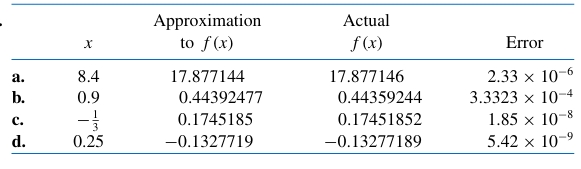
\includegraphics[width=10cm]{EndofMod3Q3sol}
\end{center}
\end{mysolution}

\item Construct the natural cubic spline for the following data.
\begin{enumerate}[label=(\alph*)]
\item
\begin{center}
\begin{tabular}{c|c}
$x$ & $f(x)$ \\
\hline
8.3 & 17.56492 \\
8.6 & 18.50515 \\
\end{tabular}
\end{center}
\item
\begin{center}
\begin{tabular}{c|c}
$x$ & $f(x)$ \\
\hline
0.8 & 0.22363362 \\
1.0 & 0.65809197 \\
\end{tabular}
\end{center}
\item
\begin{center}
\begin{tabular}{c|c}
\multicolumn{1}{c|}{$x$} & $f(x)$ \\
\hline
-0.5 & -0.0247500 \\
-0.25 & 0.3349375 \\
0 & 1.1010000 \\
\end{tabular}
\end{center}
\item
\begin{center}
\begin{tabular}{c|r}
$x$ & \multicolumn{1}{|c}{$f(x)$} \\
\hline
0.1 & -0.62049958 \\
0.2 & -0.28398668 \\
0.3 & 0.00660095 \\
0.4 & 0.24842440 \\
\end{tabular}
\end{center}
\end{enumerate}
\begin{mysolution}
The equations of the respective free cubic splines are
\[S(x)=S_i(x)=a_i+b_i(x-x_i)+c_i(x-x_i)^2+d_i(x-x_i)^3,\]
for $x$ in $[x_i, x_{i+1}]$, where the coefficients are given in the following tables.
\begin{enumerate}[label=(\alph*)]
\item ~
\begin{center}
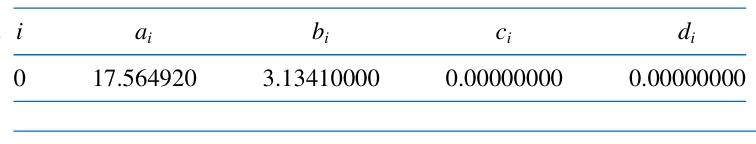
\includegraphics[width=10cm]{EndofMod3Q4sola}
\end{center}
\item ~
\begin{center}
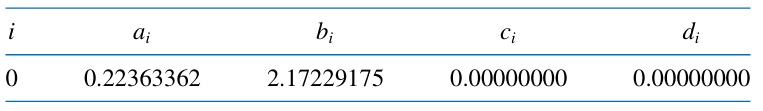
\includegraphics[width=10cm]{EndofMod3Q4solb}
\end{center}
\item ~
\begin{center}
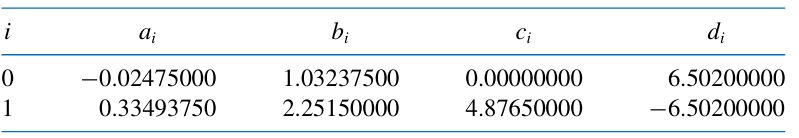
\includegraphics[width=10cm]{EndofMod3Q4solc}
\end{center}
\item ~
\begin{center}
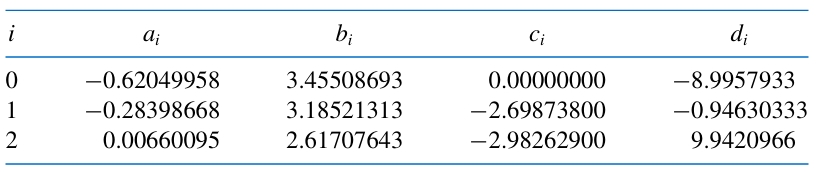
\includegraphics[width=10cm]{EndofMod3Q4sold}
\end{center}
\end{enumerate}
\end{mysolution}
\end{posttest}
%share your understanding of properties of functions and their applications to solving rates of change problems in physical phenomenon 


%\end{actsoln}

\takehome

\comy{You are now at the last part of this module. Your  task is to do a self-reflection on your learning experience.}



\references
\begin{refenumerate}
\item Kong, Q., Siauw, T., Bayen, A., (2020). Python Programming and Numerical Methods. First Edition, Academic Press,  ISBN-13 ‏ : ‎ 978-0128195499 \\
%chapter 1 pg 7-36 functions\\
%chapter 1 pg 51-83 limits and continuity\\
%chapter 1 pg 45-50 rates of change\\
%chapter 2 pg 108-120 the derivative\\
%\item Mendelson, E. (2022). Schaum's Outline of Calculus. McGraw-Hill Education.
%chapter 6 51-55 functions
%chapter 7 59-65 limits
%chapter 8 69-74 continuity
%chapter 9 77-81 derivative
%\item Calculus \mylink{https://math.libretexts.org/Bookshelves/Calculus}
%\item Chris McMullen, 2021, Essential Calculus Skills Practice Workbook with Full Solutions, Zishka Publishing, ISBN 978-1-941691-24-3
%\item R. Adams and C. Essex, 2021, Calculus: A complete Course, Addison Wesley, ISBN 13: 978-0135732588
%\item P. Abbott and H. Neill, 2018, Calculus: A Complete Introduction: The Easy Way to Learn Calculus (Teach Yourself), ISBN 13: 978-1473678446
\end{refenumerate}





%\wrapup
%To wrap-up, answer the following questions:
%
%\begin{enumerate}
%\item 
%%when do we say that a limit of a function exists?
%%\item how do we remove discontinuity in functions?
%%\item what is the relationship between the gradient of the tangent line and the derivative?
%\end{enumerate}
















%\newpage

%\facilitation


%
\begin{center}
    {\Large \textbf{FUNCTIONS OF SEVERAL VARIABLES}}\\[2mm]
(DEFINITION, DOMAIN, RANGE, GRAPHS AND LEVEL CURVES) \\[4mm]

\mycenterbox{5 minute review}%\\[4mm]
Recap the definition of a function of several variables, and the meaning of domain, range, graph and level curves of functions of several variables.
\end{center}
\mycenterbox{Warm-up.}%\\[4mm]
\problemAnswer{
Match the function with its graph (labeled I–VI).Give reasons for your choices
\begin{multicols}{3}
\begin{enumerate}[label=(\alph*)]
\item $f(x,y)=|x|+|y|$\\[4mm]
\item $f(x,y)=|xy|$
\item $f(x,y)=\frac{1}{1+x^2+y^2}$\\2mm]
\item $f(x,y)=(x^2-y^2)^2$
\item $f(x,y)=(x-y)^2$\\[4mm]
\item $f(x,y)=\sin(|x|+|y|)$
\end{enumerate}
\end{multicols}

\begin{center}
%\centering
\includegraphics[width=10cm]{MCTutorial1Q1.JPEG}
\end{center}
%\tcbox[tcbox raise base]{Warm-up}
 
%\begin{flushright}
%\begin{tikzpicture}
%    % A body
%
%
%    % Non-rectangle shapes must be drawn as polygone
%    \begin{scope}[shift={(3,0)}]
%        \draw  (0,0.5) -- (0,4) -- (.5,4) -- (.5,4.5) -- (1.,4.5) -- (4.,4.5) --(4.,4)-- (4.5,4) --(4.5,0.5) --(4.0,0.5)--(4.0,0.0)-- (.5,0) --(0.5,0.5) -- cycle;
%        % Draw symmetry lines
%        \draw [symmetry] (.5, 0.5) -- (.5,4.0);
%        \draw [symmetry] (4, 0.5) -- (4,4.0);
%        \draw [symmetry] (.5,4.0) -- (4,4.0);
%         \draw [symmetry] (.5, 0.5) -- (4, 0.5);
%        % Dimensions
%        \draw (4.5,0) -- ++(0.5,0) coordinate (D1) -- +(5pt,0);
%        \draw (4.5,4.5) -- ++(0.5,0) coordinate (D2) -- +(5pt,0);
%        \draw [dimen] (D1) -- (D2) node {6cm};
%       
%        
%        \draw (0.0,5) -- ++(0,0.5) coordinate (D1) -- +(0,+5pt);
%        \draw (0.5,5) -- ++(0,0.5) coordinate (D2) -- +(0,+5pt);
%        \draw [dimen,-] (D1) -- (D2) node [above=5pt] {$x$ cm};
%        \draw [dimen,<-] (D1) -- ++(-5pt,0);
%        \draw [dimen,<-] (D2) -- ++(+5pt,0);
%    \end{scope}
%\end{tikzpicture}
%\end{flushright}

}


\mycenterbox{Problems.}%

%\begin{center}
%\tcbox[tcbox raise base]{ Problems. Choose from the below}
%\end{center}
\problem{Exploring functions}%
\begin{enumerate}[(a)]
\item Are the following functions even, odd, or neither? What can you say
about their range?
\begin{multicols}{4}
 \begin{enumerate}[(i)]
\item $\displaystyle \frac{3x}{x^2+2}$
\item $\displaystyle \cos x+3$
\item $\displaystyle \frac{2x^3}{\cos x+3}$
\item $\displaystyle \frac{3x^4+2x^2}{\sin x+4}$
\end{enumerate}
\end{multicols}
\item Consider the functions $\sin^n x$ and $\cos^n x$, where $n$ is a positive integer.
Which are odd, which are even, and what are their periodicities?
\item What is the periodicity of $f(x) = 2 \cos x+\sin 2x$? Is it even/odd/neither?

\end{enumerate}

\problem{Cubic functions} 
Show that $x-1$ is a factor of the cubic function%
$$P(x)=x^3-2x^2-5x+6,$$
and  find the quadratic factor $Q(x)$ such that $P(x) = (x -1)Q(x)$. Factorise
$Q(x)$ and hence sketch $P(x).$

%\newpage
\problem{Sigmoid functions*.}%
For positive integers $n$, consider the family of functions
$$\displaystyle f_n= \frac{x^n}{2^n+x^n}.$$
\begin{enumerate}[(a)]
\item What are appropriate domains and ranges for $f_n(x)$? Do they depend on $n$?

\item Is $f_n(x)$ even, odd, or neither? Does this depend on $n$?

\item Show that for $x\geq 0$, $f_n(x)$ are strictly increasing functions and that
$0\leq f_n(x) < 1.$
\item What is the value of $f_n(2)$? Does it depend on $n$?

\item By considering the values of $f_n(1.9)$ and $f_n(2.1)$ for $n = 2, 4, 8, 16, 32$ and
$64$, show that the graph of $f_n(x)$ for $x\ge 0$ is an increasing sigmoid (that
is, $S$-shaped) function that approaches a step function as $n\rightarrow \infty$.
\end{enumerate}

\mycenterbox{Selected answers and hints}%

For the warm-up, $V(x)=4x(3-x)^2$. Writing $x=1+\epsilon$, we get
$$V = 4(1 +\epsilon)(3- (1+\epsilon))^2=4(4-\epsilon^2(3-\epsilon)).$$
If $-1<\epsilon<2$ then $\epsilon^2 (3-\epsilon)\ge 0$, with equality when $\epsilon=0$. Thus the maximum
value of $V$ occurs when $\epsilon= 0$, i.e. $x = 1\rm{cm}$.

\begin{enumerate}
\item 
\begin{enumerate}[(i)]
\item Odd. The range is the interval  $[-\frac{3}{4}\sqrt{2},\; \frac{3}{4}\sqrt{2}]$
\item Even. The range is the interval $[2, 4]$.
\item Odd. The range is all of $\mathbb R$.
\item Neither. (For example, writing $\displaystyle \frac{5}{\sin x+4}$ we have $\displaystyle f(1)= \frac{5}{\sin (1)+4} \equiv 1.032 (3\rm{dp})$ which is neither $f(1)$ nor $-f(1)$.)\\[4mm]
The range is the nonnegative reals $[0,\infty)$

\end{enumerate}
\end{enumerate}










